\documentclass[11pt]{amsart}

\usepackage[a4paper,margin=2.35cm]{geometry}
\usepackage[T1]{fontenc}
\usepackage[utf8]{inputenc}
\usepackage[english]{babel}
\usepackage{amsmath}
\usepackage{amssymb}
\usepackage{amsthm}
\usepackage{amsfonts}
\usepackage{mathtools}
\usepackage{bm}
\usepackage{booktabs}
\usepackage{longtable}
\usepackage{array}
\usepackage{graphicx}
\usepackage{microtype}
\usepackage{enumitem}
\usepackage{caption}
\usepackage{subcaption}
\usepackage{placeins}
\usepackage{xcolor}
\usepackage[hidelinks]{hyperref}

\numberwithin{equation}{section}

\newtheorem{theorem}{Theorem}[section]
\newtheorem{proposition}[theorem]{Proposition}
\newtheorem{lemma}[theorem]{Lemma}
\newtheorem{corollary}[theorem]{Corollary}
\newtheorem{conjecture}[theorem]{Conjecture}
\theoremstyle{definition}
\newtheorem{definition}[theorem]{Definition}
\theoremstyle{remark}
\newtheorem{remark}[theorem]{Remark}

\newcommand{\dd}{\,\mathrm d}
\newcommand{\R}{\mathbb R}
\newcommand{\C}{\mathbb C}
\newcommand{\Chat}{\widehat{\mathbb C}}
\newcommand{\Ree}{\operatorname{Re}}
\newcommand{\Imm}{\operatorname{Im}}
\newcommand{\sgn}{\operatorname{sgn}}
\newcommand{\ord}{\operatorname{ord}}
\newcommand{\Sch}{\mathcal S}
\newcommand{\Ical}{\mathcal I}
\newcommand{\Hcal}{\mathcal H}
\newcommand{\Pcal}{\mathcal P}
\newcommand{\Ccal}{\mathcal C}

\setlength{\textfloatsep}{10pt plus 2pt minus 2pt}
\setlength{\floatsep}{8pt plus 2pt minus 2pt}
\setlength{\intextsep}{8pt plus 2pt minus 2pt}
\renewcommand{\topfraction}{0.92}
\renewcommand{\bottomfraction}{0.85}
\renewcommand{\textfraction}{0.07}
\renewcommand{\floatpagefraction}{0.78}
\captionsetup{font=small}
\raggedbottom

\title[Euclidean lobe geometry of the zeta function]{Euclidean Lobe Geometry, Reciprocal Scattering, and Transverse Projective Structure of the Riemann Zeta Function}
\author{Víctor Casaña-Giner}
\address{Bio Logic Crop Science S.L.}
\thanks{ORCID: 0000-0002-8252-2608}
\subjclass[2020]{11M26, 30C55, 30F45}
\keywords{Riemann zeta function, zero-to-zero lobes, Riemann--Siegel phase, reciprocal geometry, Schwarzian derivative, Lambert W, transverse flow}
\date{25 August 2026}

\begin{document}

\begin{abstract}
The curve
\begin{equation}
\Gamma(t)=\left(t,\Ree\zeta\!\left(\tfrac12+it\right),\Imm\zeta\!\left(\tfrac12+it\right)\right)
\label{eq:abstract-thread}
\end{equation}
is treated as a primary Euclidean object and decomposed into zero-to-zero lobes.  The construction combines radial excursion, angular sweep, Euclidean arc length, eccentric lobe geometry, reciprocal scattering, and the exact transverse equation
\begin{equation}
F_\delta=-iF_t,
\qquad
F(\delta,t)=\zeta\!\left(\tfrac12+\delta+it\right).
\label{eq:abstract-quarter-turn}
\end{equation}
The Riemann--von Mangoldt/Lambert phase produces an exact tangent-circle model whose reciprocal image is a straight scattering branch and whose transverse continuation satisfies an explicit no-exit theorem.  For the exact zeta lobes we derive a reciprocal normal form, a corrected endpoint scattering cocycle, and a projective defect based on the Schwarzian derivative.  The sign and reciprocal conventions in the endpoint jet formulas are fixed explicitly: the relevant quotient is $w_n'(1)/w_n'(0)$, not its reciprocal, and the cocycle potential is $Q_n=-\log a_n-i\psi_n$.

The projective block yields an exact second-order equation, an exact closure orthogonality, an exact complex moment formula for the endpoint jet holonomy, and a telescoping product law.  These identities are structural rather than a confinement proof: no independent inequality forcing zero-exclusion is obtained from the Schwarzian alone.  The reciprocal chart $U=1/F$ is also treated with its exact logical status: a pole of $U$ and a zero of $F$ are the same event at the same domain point.  Its utility is methodological, not logical, because a lower-bound problem for $|F|$ becomes an upper-bound problem for $|U|$ only on regions where the reciprocal chart is already holomorphic.

The numerical figures and tables carried into this version are unchanged from the preceding verified computation.  Version 5 is an analytic and typographical revision; the binary corpus was not re-inspected or recomputed.
\end{abstract}

\maketitle
\tableofcontents

\section{Status and scope}
\label{sec:status}

The purpose of this paper is to retain one geometric object throughout: the trace in \eqref{eq:abstract-thread}, referred to as the \emph{Violet Thread}.  The main statements are separated by mathematical status.

\begin{proposition}[Exact structural layer]
\label{prop:status-exact}
The following statements are exact consequences of the definitions used below: the zero-to-zero lobe decomposition, the Hardy-frame speed identity, the transverse quarter-turn equation \eqref{eq:abstract-quarter-turn}, the RVM tangent-circle identity, the RVM reciprocal straight-line identity, the RVM no-exit theorem, the reciprocal curvature formula, the corrected scattering cocycle, the endpoint-normalized lobe factorization, and the Schwarzian closure and holonomy identities.
\end{proposition}

\begin{remark}[Logical status of transverse confinement]
\label{rem:status-rh}
The assertion
\begin{equation}
F(\delta,t)\neq0
\quad\text{for every }t\in\R\text{ and }0<|\delta|<\tfrac12
\label{eq:global-no-exit}
\end{equation}
is exactly the desired global zero-confinement statement.  Equation \eqref{eq:abstract-quarter-turn} is a complete first-order evolution equation, so a proof of \eqref{eq:global-no-exit} from a global invariant of that first-order field would require no subsequent hierarchy of second-, third-, or higher-order conditions.  Equation \eqref{eq:abstract-quarter-turn} by itself does not prove \eqref{eq:global-no-exit}.
\end{remark}

\begin{remark}[Numerical layer]
\label{rem:status-numerical}
The reported correlations for the first 49 lobes and the full $2{,}001{,}052$-ordinate phase/RVM summaries are carried unchanged from the preceding verified computation.  They are not recomputed in Version 5.
\end{remark}

\section{Notation}
\label{sec:notation}

\begin{center}
\small
\begin{tabular}{>{\raggedright\arraybackslash}p{0.22\textwidth}p{0.70\textwidth}}
\toprule
Symbol & Meaning \\
\midrule
$W(t)$ & $\zeta(\tfrac12+it)$, the complex value trace of the Violet Thread \\
$\Gamma(t)$ & $(t,\Ree W(t),\Imm W(t))\in\R^3$ \\
$Z(t)$ & Hardy's real function, $W(t)=Z(t)e^{-i\vartheta(t)}$ \\
$\vartheta(t)$ & Riemann--Siegel phase \\
$\gamma_n$ & successive zeros of $W$ on the central trace \\
$I_n$ & $(\gamma_n,\gamma_{n+1})$ \\
$g_n$ & $\gamma_{n+1}-\gamma_n$ \\
$\Omega_n$ & $\vartheta(\gamma_{n+1})-\vartheta(\gamma_n)$ \\
$s_n$ & $\Omega_n/\pi$ \\
$A_n$ & $\max_{I_n}|Z(t)|$ \\
$L_n$ & Euclidean arc length of the $n$th lobe \\
$R_n$ & $L_n/g_n$ \\
$F(\delta,t)$ & $\zeta(\tfrac12+\delta+it)$ \\
$U(\delta,t)$ & reciprocal chart $1/F(\delta,t)$ where defined \\
$\Theta_0$ & smooth RVM phase $\frac z2\log(z/(2\pi e))-\frac\pi8$ \\
$\tau_n$ & RVM/Lambert ordinates \\
$\Ccal_n$ & phase centroid of a rotated lobe \\
$E_n$ & normalized eccentricity $2|\Ccal_n|/A_n$ \\
$D_n$ & normalized circle-tangency defect \\
$\Hcal_n$ & endpoint jet quotient $w_n'(1)/w_n'(0)$ \\
$Q_n$ & corrected scattering potential $-\log a_n-i\psi_n$ \\
$\Pcal_n$ & projective lobe defect $\{w_n,q\}-2\pi^2$ \\
\bottomrule
\end{tabular}
\end{center}

\section{The Violet Thread and its zero-to-zero lobes}
\label{sec:thread}

\begin{definition}[Violet Thread]
\label{def:thread}
Define
\begin{equation}
W(t)=\zeta\!\left(\frac12+it\right)=u(t)+iv(t),
\label{eq:W-definition}
\end{equation}
and
\begin{equation}
\Gamma(t)=\bigl(t,u(t),v(t)\bigr).
\label{eq:Gamma-definition}
\end{equation}
\end{definition}

The classical Hardy decomposition \cite{Titchmarsh1986,Edwards2001} is
\begin{equation}
W(t)=Z(t)e^{-i\vartheta(t)},
\qquad Z(t)\in\R.
\label{eq:Hardy-decomposition}
\end{equation}
Consequently
\begin{equation}
\Gamma(t)=\bigl(t,Z(t)\cos\vartheta(t),-Z(t)\sin\vartheta(t)\bigr).
\label{eq:cylindrical-thread}
\end{equation}
Differentiation gives
\begin{equation}
W_t(t)=e^{-i\vartheta(t)}\bigl(Z'(t)-i\vartheta'(t)Z(t)\bigr)
\label{eq:Wt-Hardy}
\end{equation}
and hence
\begin{equation}
|W_t(t)|^2=Z'(t)^2+\vartheta'(t)^2Z(t)^2.
\label{eq:speed-Hardy}
\end{equation}

\begin{figure}[tbp]
\centering
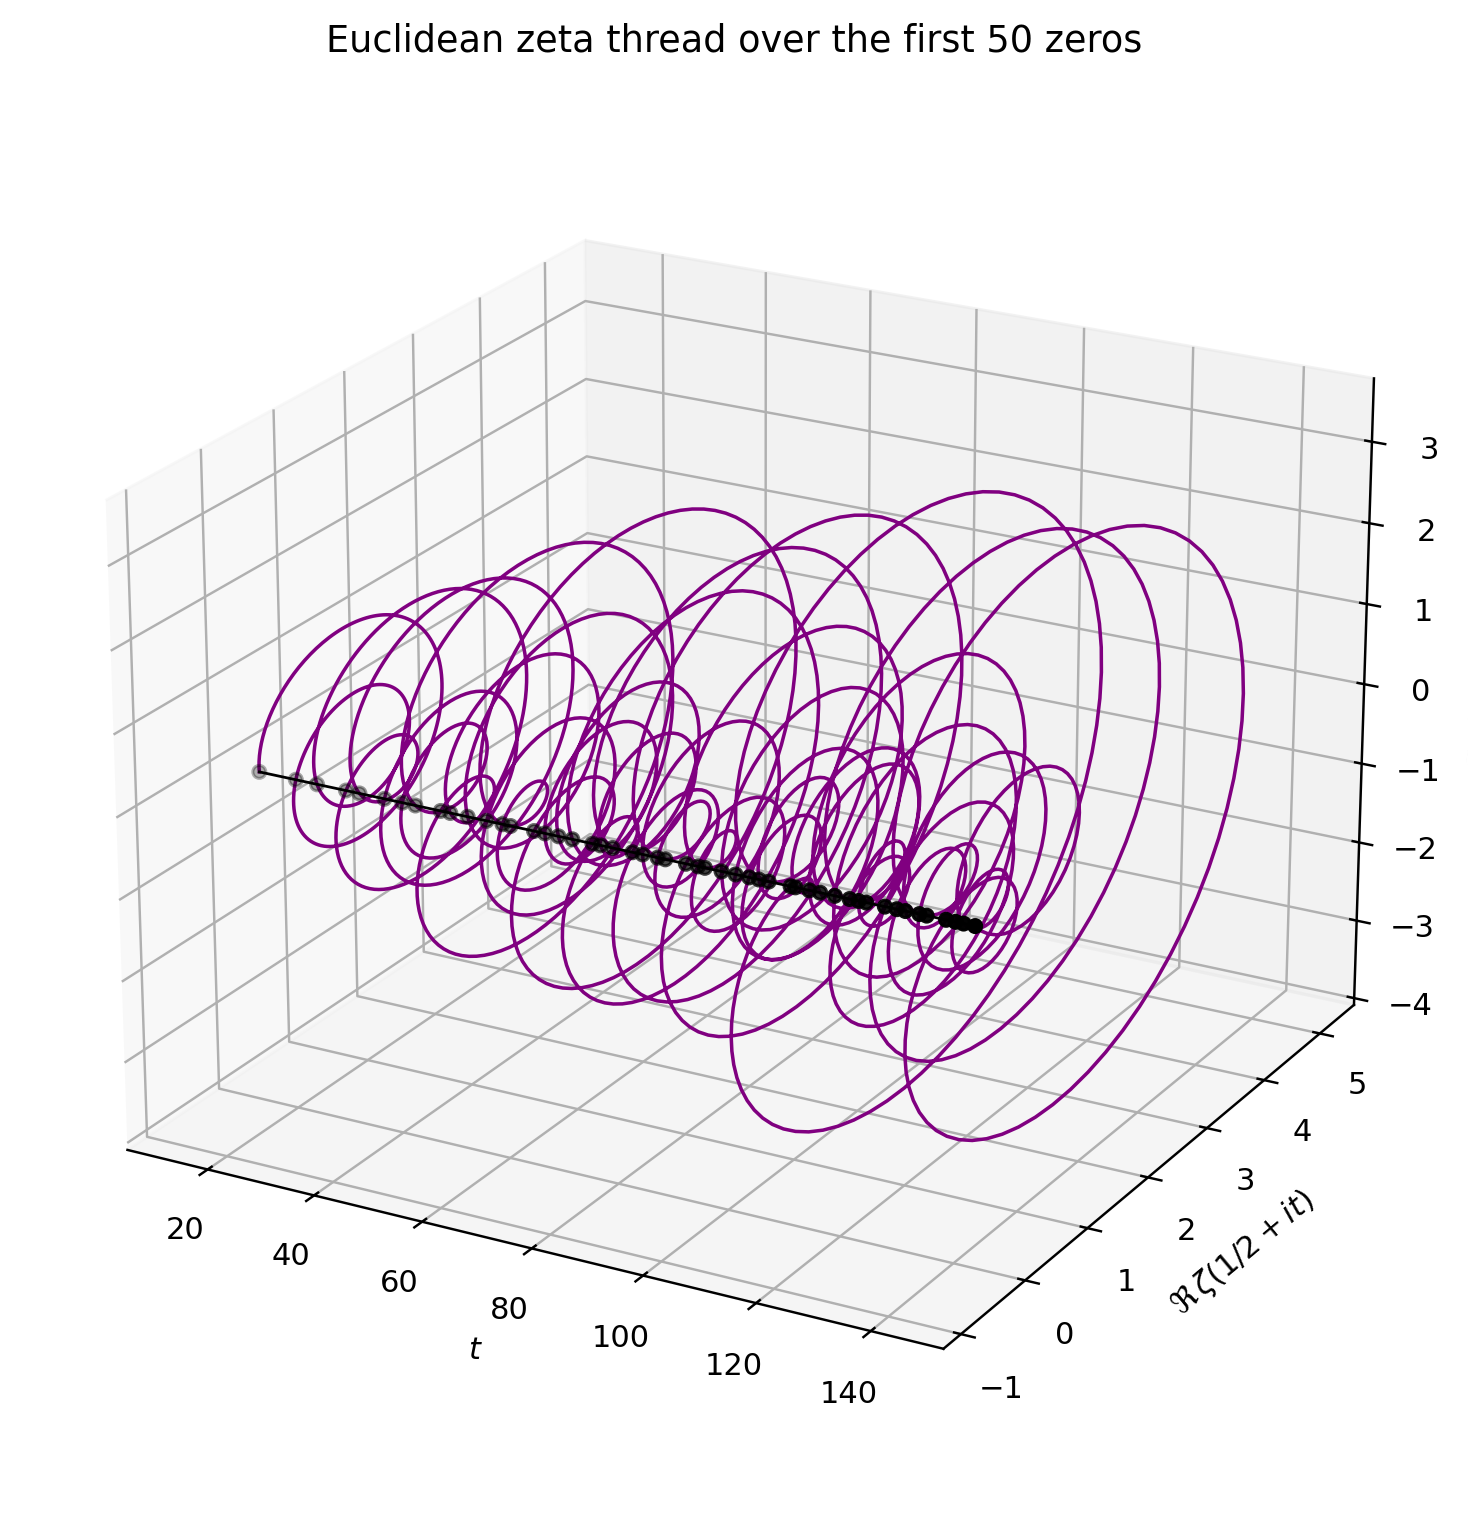
\includegraphics[width=.70\textwidth]{../figures/fig01_euclidean_zeta_thread.png}
\caption{The Euclidean Violet Thread over the first fifty carried zero ordinates.  Height remains an explicit coordinate, so the transverse lobes are genuine three-dimensional curve segments.}
\label{fig:thread-3d}
\end{figure}

Let $\gamma_n<\gamma_{n+1}$ be consecutive contacts of the central trace with the value-plane origin.  On
\begin{equation}
I_n=(\gamma_n,\gamma_{n+1}),
\label{eq:lobe-interval}
\end{equation}
the sign of $Z$ is constant.  Put
\begin{equation}
\varepsilon_n=\sgn Z(t),\qquad t\in I_n,
\label{eq:epsilon-n}
\end{equation}
and rotate away the absolute initial phase:
\begin{equation}
\widehat W_n(t)=\varepsilon_n e^{i\vartheta(\gamma_n)}W(t).
\label{eq:rotated-lobe-t}
\end{equation}
Then
\begin{equation}
\widehat W_n(t)=|Z(t)|e^{-i\phi_n(t)},
\qquad
\phi_n(t)=\vartheta(t)-\vartheta(\gamma_n).
\label{eq:rotated-lobe-phase}
\end{equation}
The total angular sweep is
\begin{equation}
\Omega_n=\vartheta(\gamma_{n+1})-\vartheta(\gamma_n),
\qquad
s_n=\frac{\Omega_n}{\pi}.
\label{eq:Omega-s}
\end{equation}
Thus the usual local phase unfolding is literally the angular extent of a single lobe.

\begin{figure}[tbp]
\centering
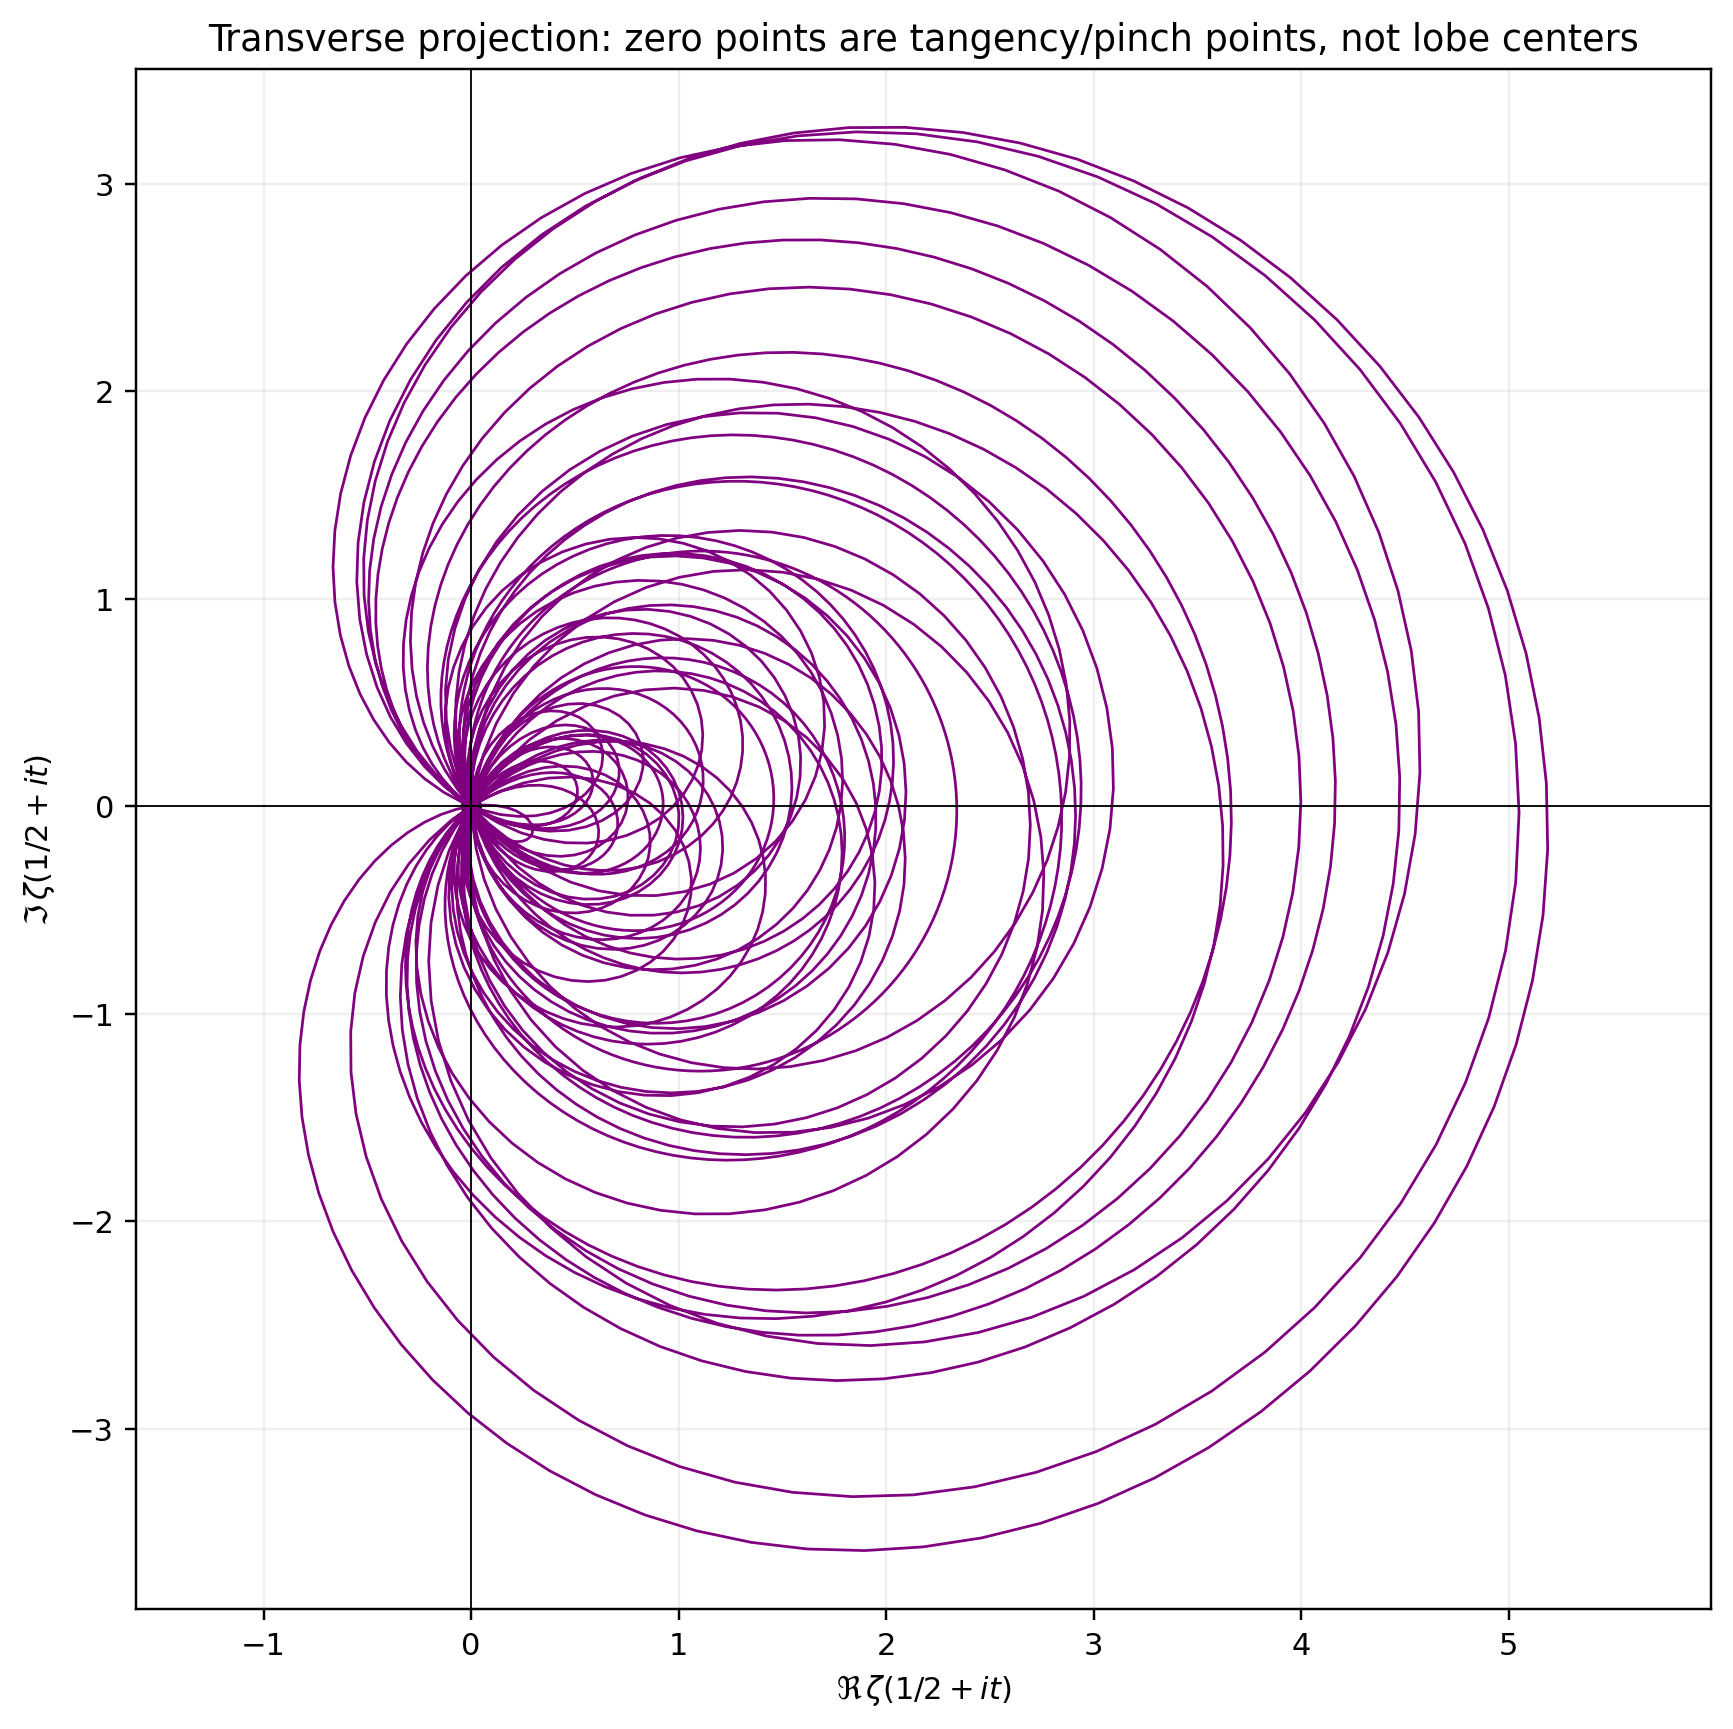
\includegraphics[width=.58\textwidth]{../figures/fig02_transverse_eccentric_lobes.png}
\caption{Transverse projection.  The common zero point is an eccentric contact of the lobes, not their geometric center.}
\label{fig:transverse-eccentricity}
\end{figure}

\section{Eccentric one-arch geometry and the RVM skeleton}
\label{sec:eccentric-rvm}

Introduce uniform phase coordinate
\begin{equation}
q=\frac{\phi_n(t)}{\Omega_n},
\qquad 0\le q\le1.
\label{eq:q-phase}
\end{equation}
The one-arch radial model retaining the measured phase sweep is
\begin{equation}
\widehat W_n^{\mathrm{arch}}(q)
=A_n\sin(\pi q)e^{-i\pi s_nq}.
\label{eq:one-arch-general}
\end{equation}

\begin{theorem}[Unit sweep is an eccentric tangent circle]
\label{thm:tangent-circle}
If $s_n=1$, then
\begin{equation}
\widehat W_n^{\mathrm{arch}}(q)
=-\frac{iA_n}{2}+\frac{iA_n}{2}e^{-2\pi iq},
\label{eq:tangent-circle-param}
\end{equation}
and therefore
\begin{equation}
\left|\widehat W_n^{\mathrm{arch}}(q)+\frac{iA_n}{2}\right|
=\frac{A_n}{2}.
\label{eq:tangent-circle-equation}
\end{equation}
The origin lies on the circle at a tangency/contact point and is not its center.
\end{theorem}

\begin{proof}
Use
\begin{equation}
\sin(\pi q)e^{-i\pi q}=\frac{1-e^{-2\pi iq}}{2i}.
\label{eq:sine-circle-identity}
\end{equation}
Substitution into \eqref{eq:one-arch-general} gives \eqref{eq:tangent-circle-param}, and \eqref{eq:tangent-circle-equation} follows.
\end{proof}

The smooth RVM phase is
\begin{equation}
\Theta_0(z)=\frac z2\log\frac{z}{2\pi e}-\frac\pi8.
\label{eq:Theta0}
\end{equation}
The Lambert representation of the corresponding ordinates is standard \cite{CorlessEtAl1996}; with the normalization used here they satisfy
\begin{equation}
\Theta_0(\tau_n)=\pi\left(n-\frac32\right).
\label{eq:tau-phase}
\end{equation}
Define the model thread
\begin{equation}
M_0(t)=\cos\Theta_0(t)e^{-i\Theta_0(t)}.
\label{eq:M0}
\end{equation}
Then
\begin{equation}
M_0(t)=\frac12\left(1+e^{-2i\Theta_0(t)}\right),
\label{eq:M0-circle}
\end{equation}
so
\begin{equation}
\left|M_0(t)-\frac12\right|=\frac12.
\label{eq:M0-circle-equation}
\end{equation}
Thus the RVM/Lambert skeleton consists of exact eccentric tangent-circle lobes.

\begin{figure}[tbp]
\centering
\begin{subfigure}[t]{.47\textwidth}
\centering
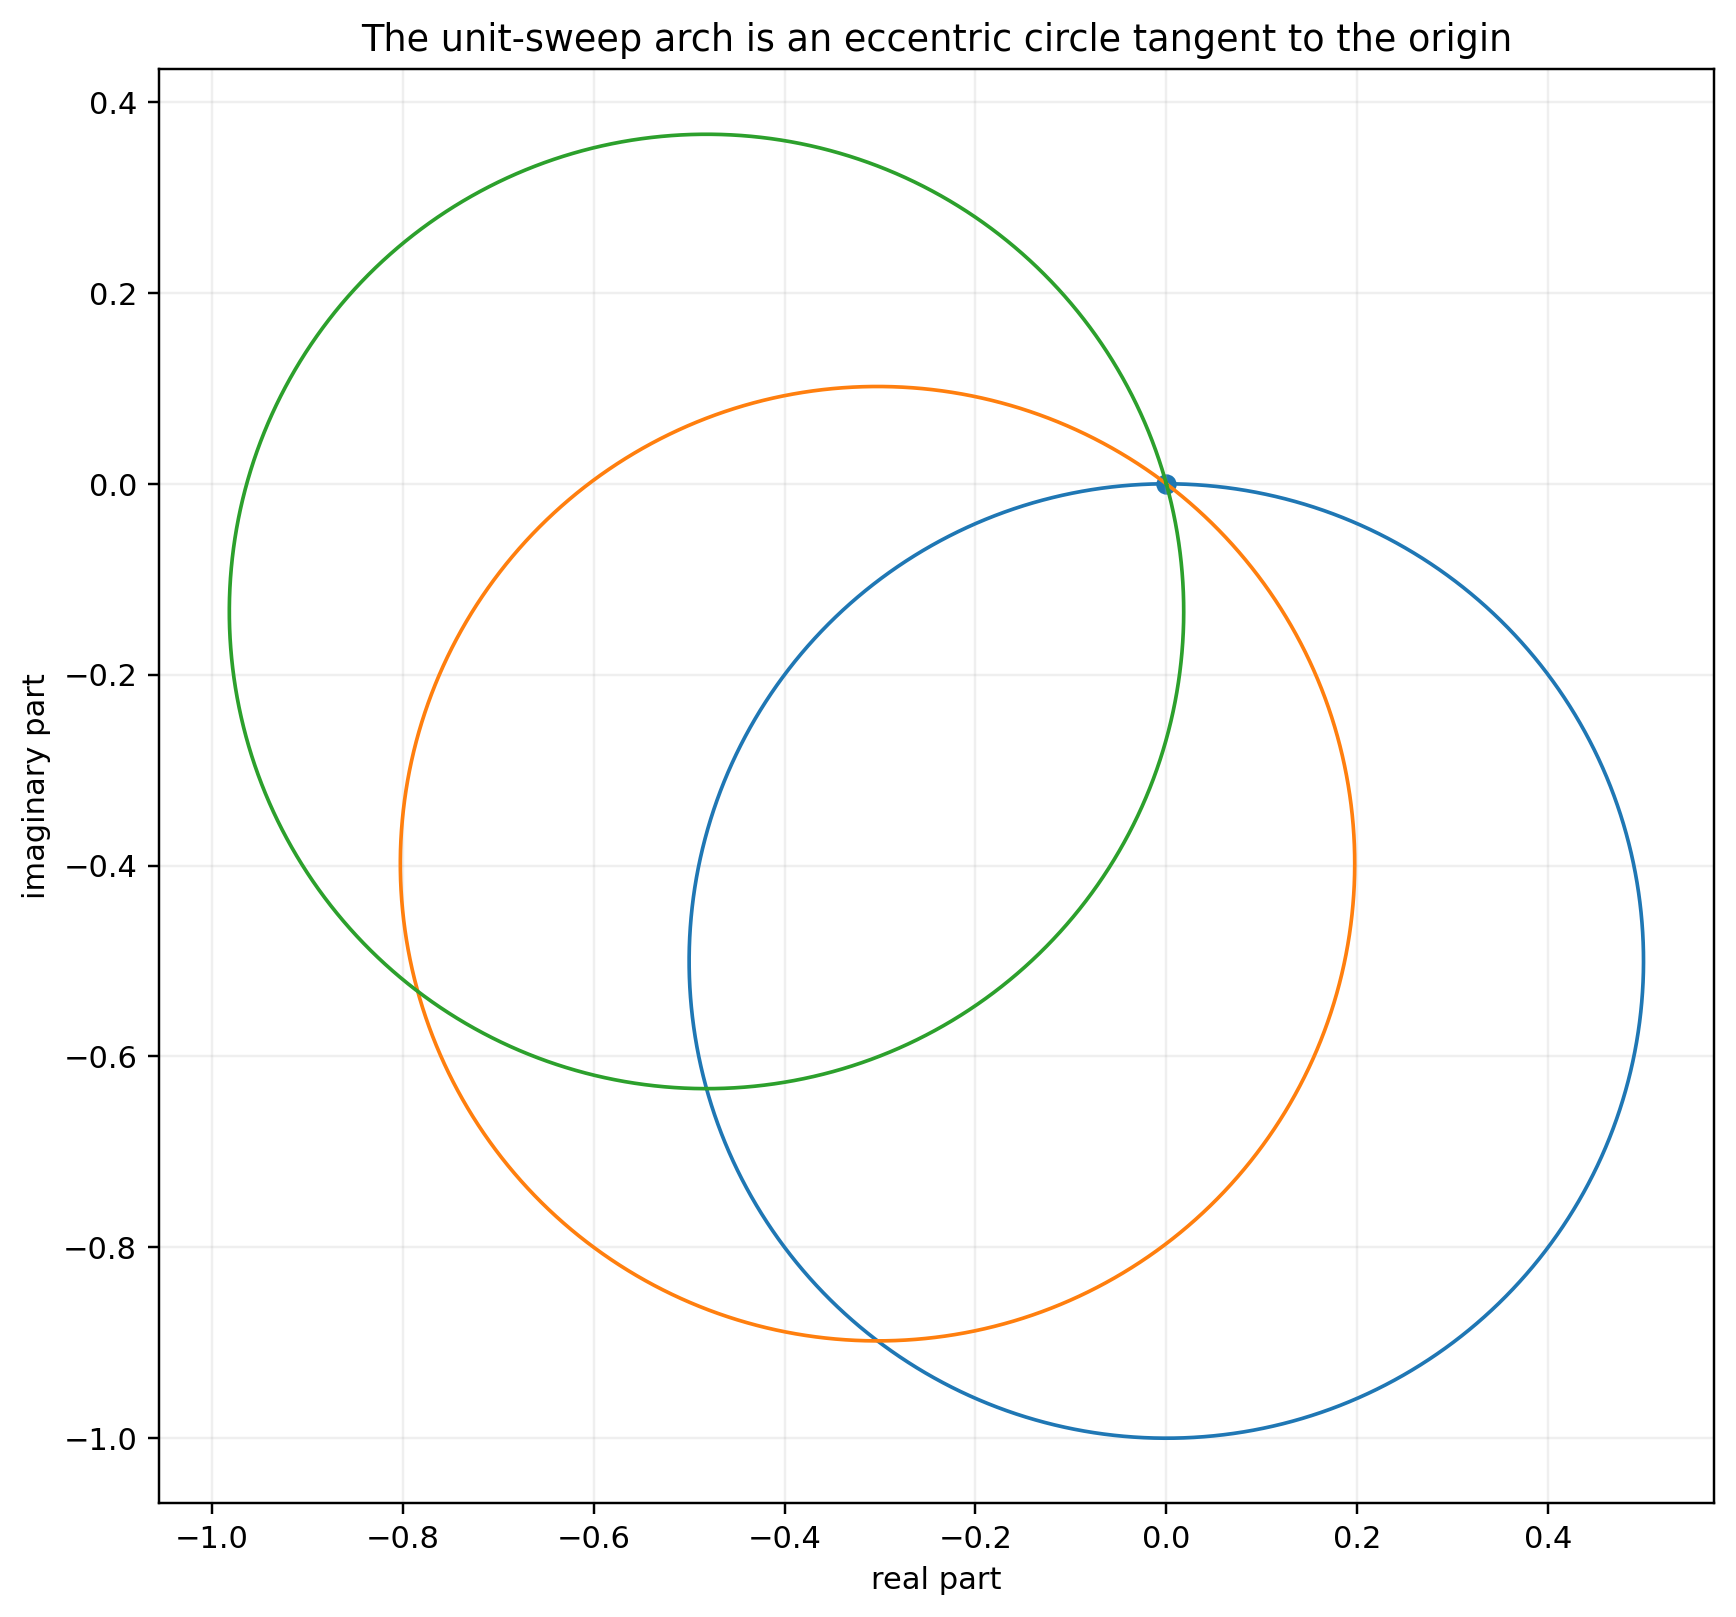
\includegraphics[width=\linewidth]{../figures/fig20_tangent_circle_identity.png}
\caption{Unit-sweep tangent-circle identity.}
\label{fig:tangent-circle-identity}
\end{subfigure}\hfill
\begin{subfigure}[t]{.47\textwidth}
\centering
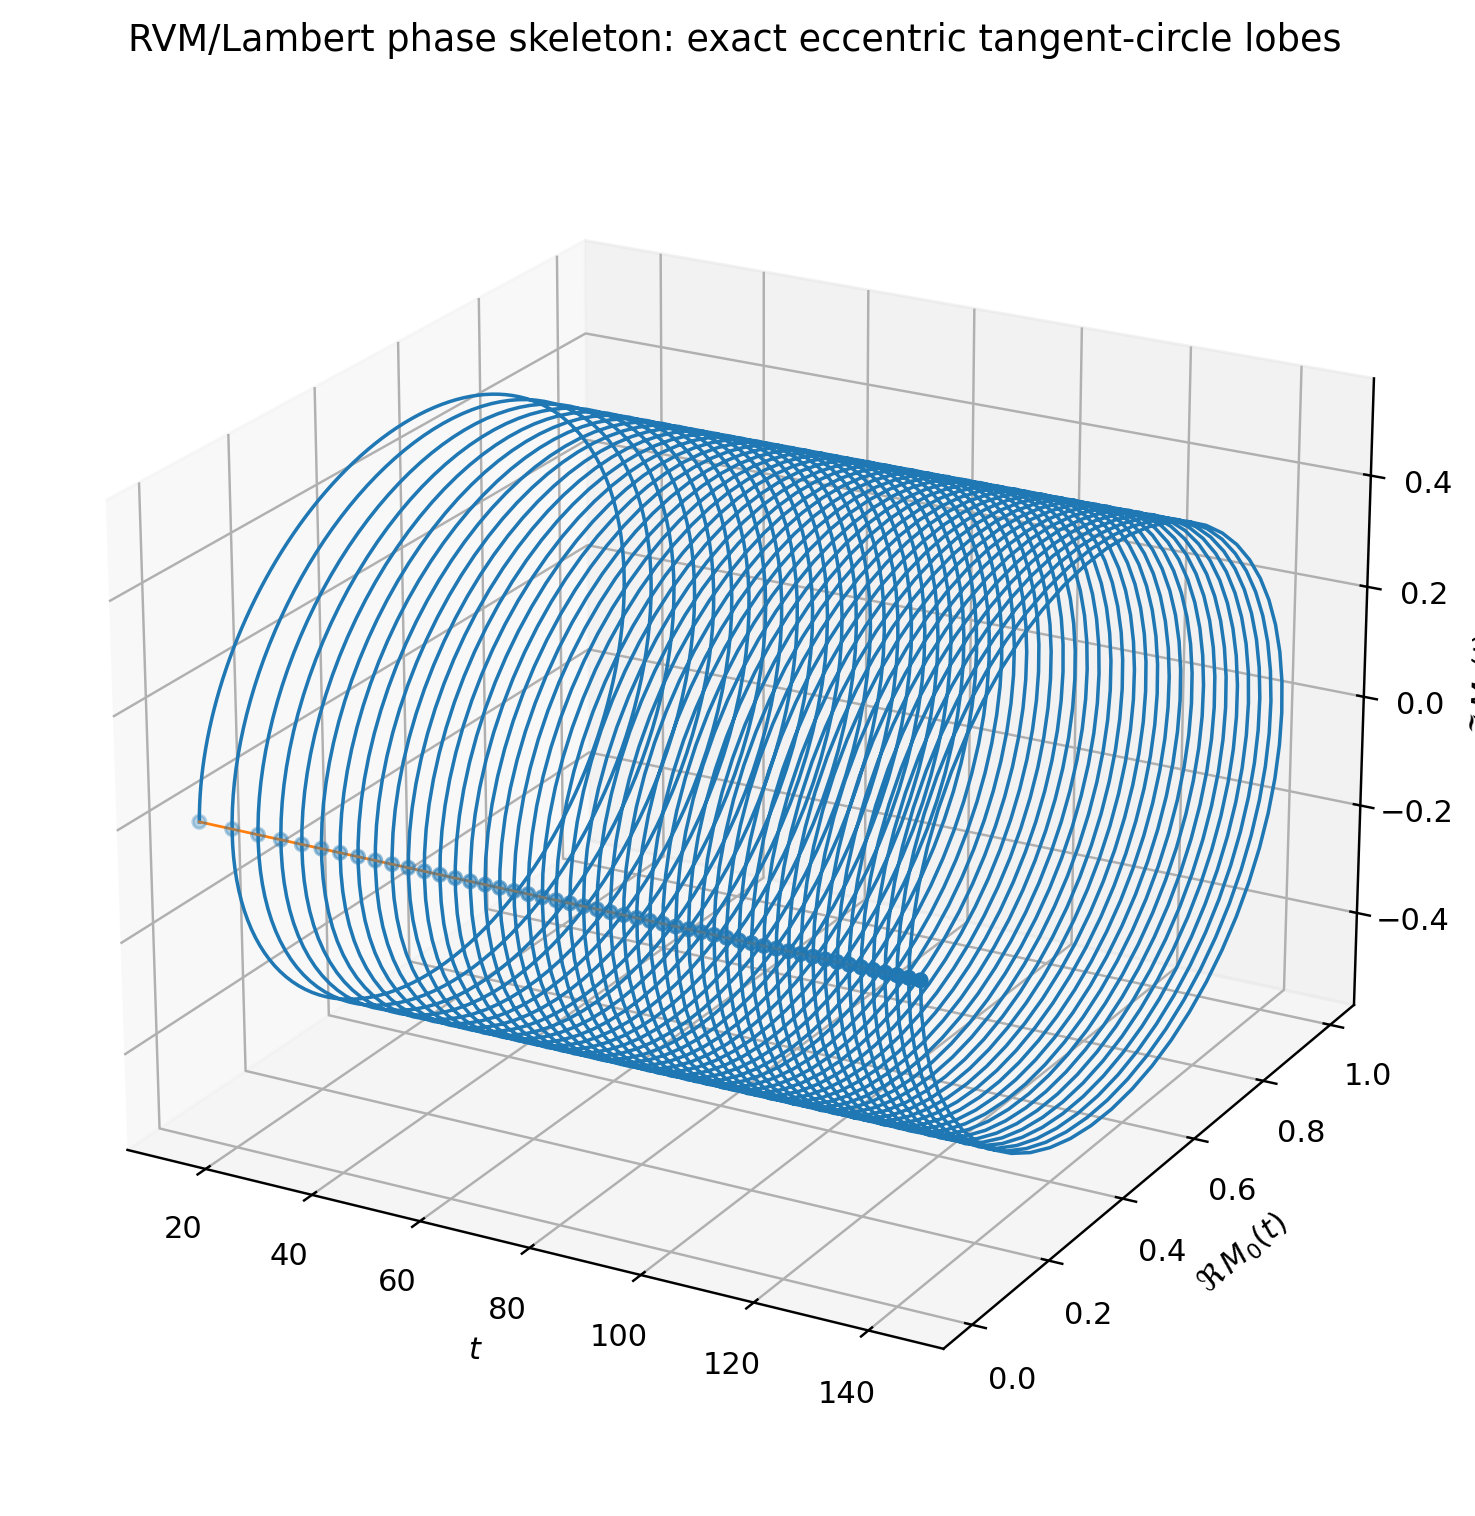
\includegraphics[width=\linewidth]{../figures/fig13_rvm_tangent_circle_thread.png}
\caption{RVM/Lambert tangent-circle skeleton.}
\label{fig:rvm-skeleton}
\end{subfigure}
\caption{The eccentric geometry generated by a unit RVM phase sweep.}
\label{fig:rvm-circle-pair}
\end{figure}

\begin{figure}[tbp]
\centering
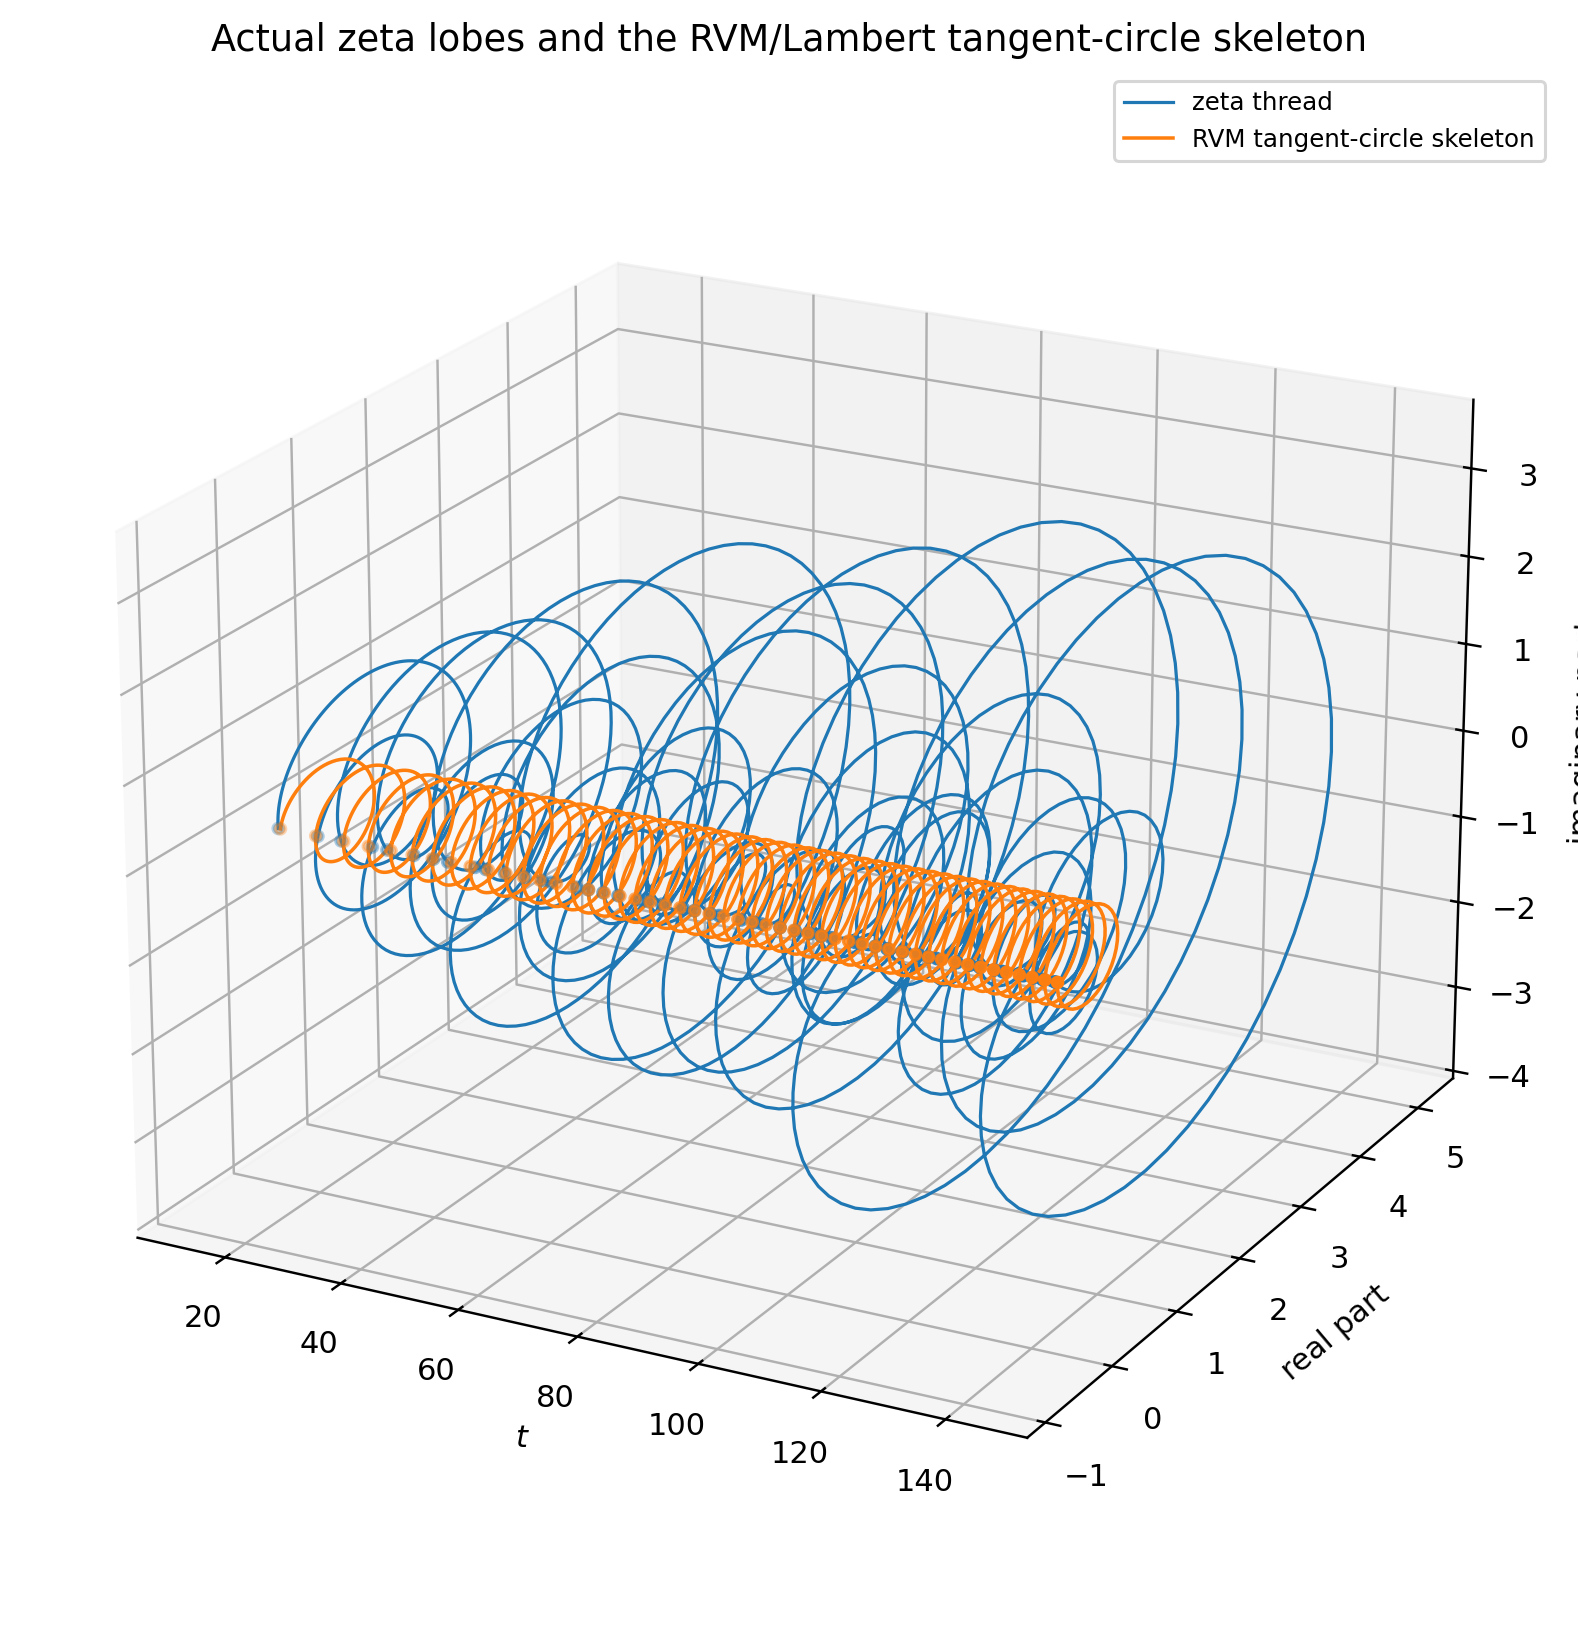
\includegraphics[width=.72\textwidth]{../figures/fig16_zeta_rvm_overlay_3d.png}
\caption{Actual zeta lobes and the RVM/Lambert tangent-circle skeleton in the same Euclidean coordinates.}
\label{fig:zeta-rvm-overlay}
\end{figure}

\section{Exact first-order transverse dynamics}
\label{sec:transverse}

Set
\begin{equation}
F(\delta,t)=\zeta\!\left(\frac12+\delta+it\right),
\qquad -\frac12<\delta<\frac12.
\label{eq:F-definition}
\end{equation}

\begin{theorem}[Global quarter-turn equation]
\label{thm:quarter-turn}
The complete transverse family satisfies
\begin{equation}
F_\delta(\delta,t)=-iF_t(\delta,t).
\label{eq:quarter-turn}
\end{equation}
In the value plane the transverse and longitudinal velocities are orthogonal and have equal magnitude.
\end{theorem}

\begin{proof}
If $s=\tfrac12+\delta+it$, then
\begin{equation}
F_\delta=\zeta'(s),
\qquad
F_t=i\zeta'(s),
\label{eq:F-derivatives}
\end{equation}
which gives \eqref{eq:quarter-turn}.
\end{proof}

On the central thread, \eqref{eq:Wt-Hardy} gives
\begin{equation}
F_\delta(0,t)=e^{-i\vartheta(t)}\bigl(-\vartheta'(t)Z(t)-iZ'(t)\bigr).
\label{eq:transverse-Hardy}
\end{equation}
Thus the Hardy frame separates the transverse generator into radial and angular components:
\begin{equation}
N_{\mathrm{rad}}(t)=-\vartheta'(t)Z(t),
\qquad
N_{\mathrm{ang}}(t)=-Z'(t).
\label{eq:normal-components}
\end{equation}

\begin{figure}[tbp]
\centering
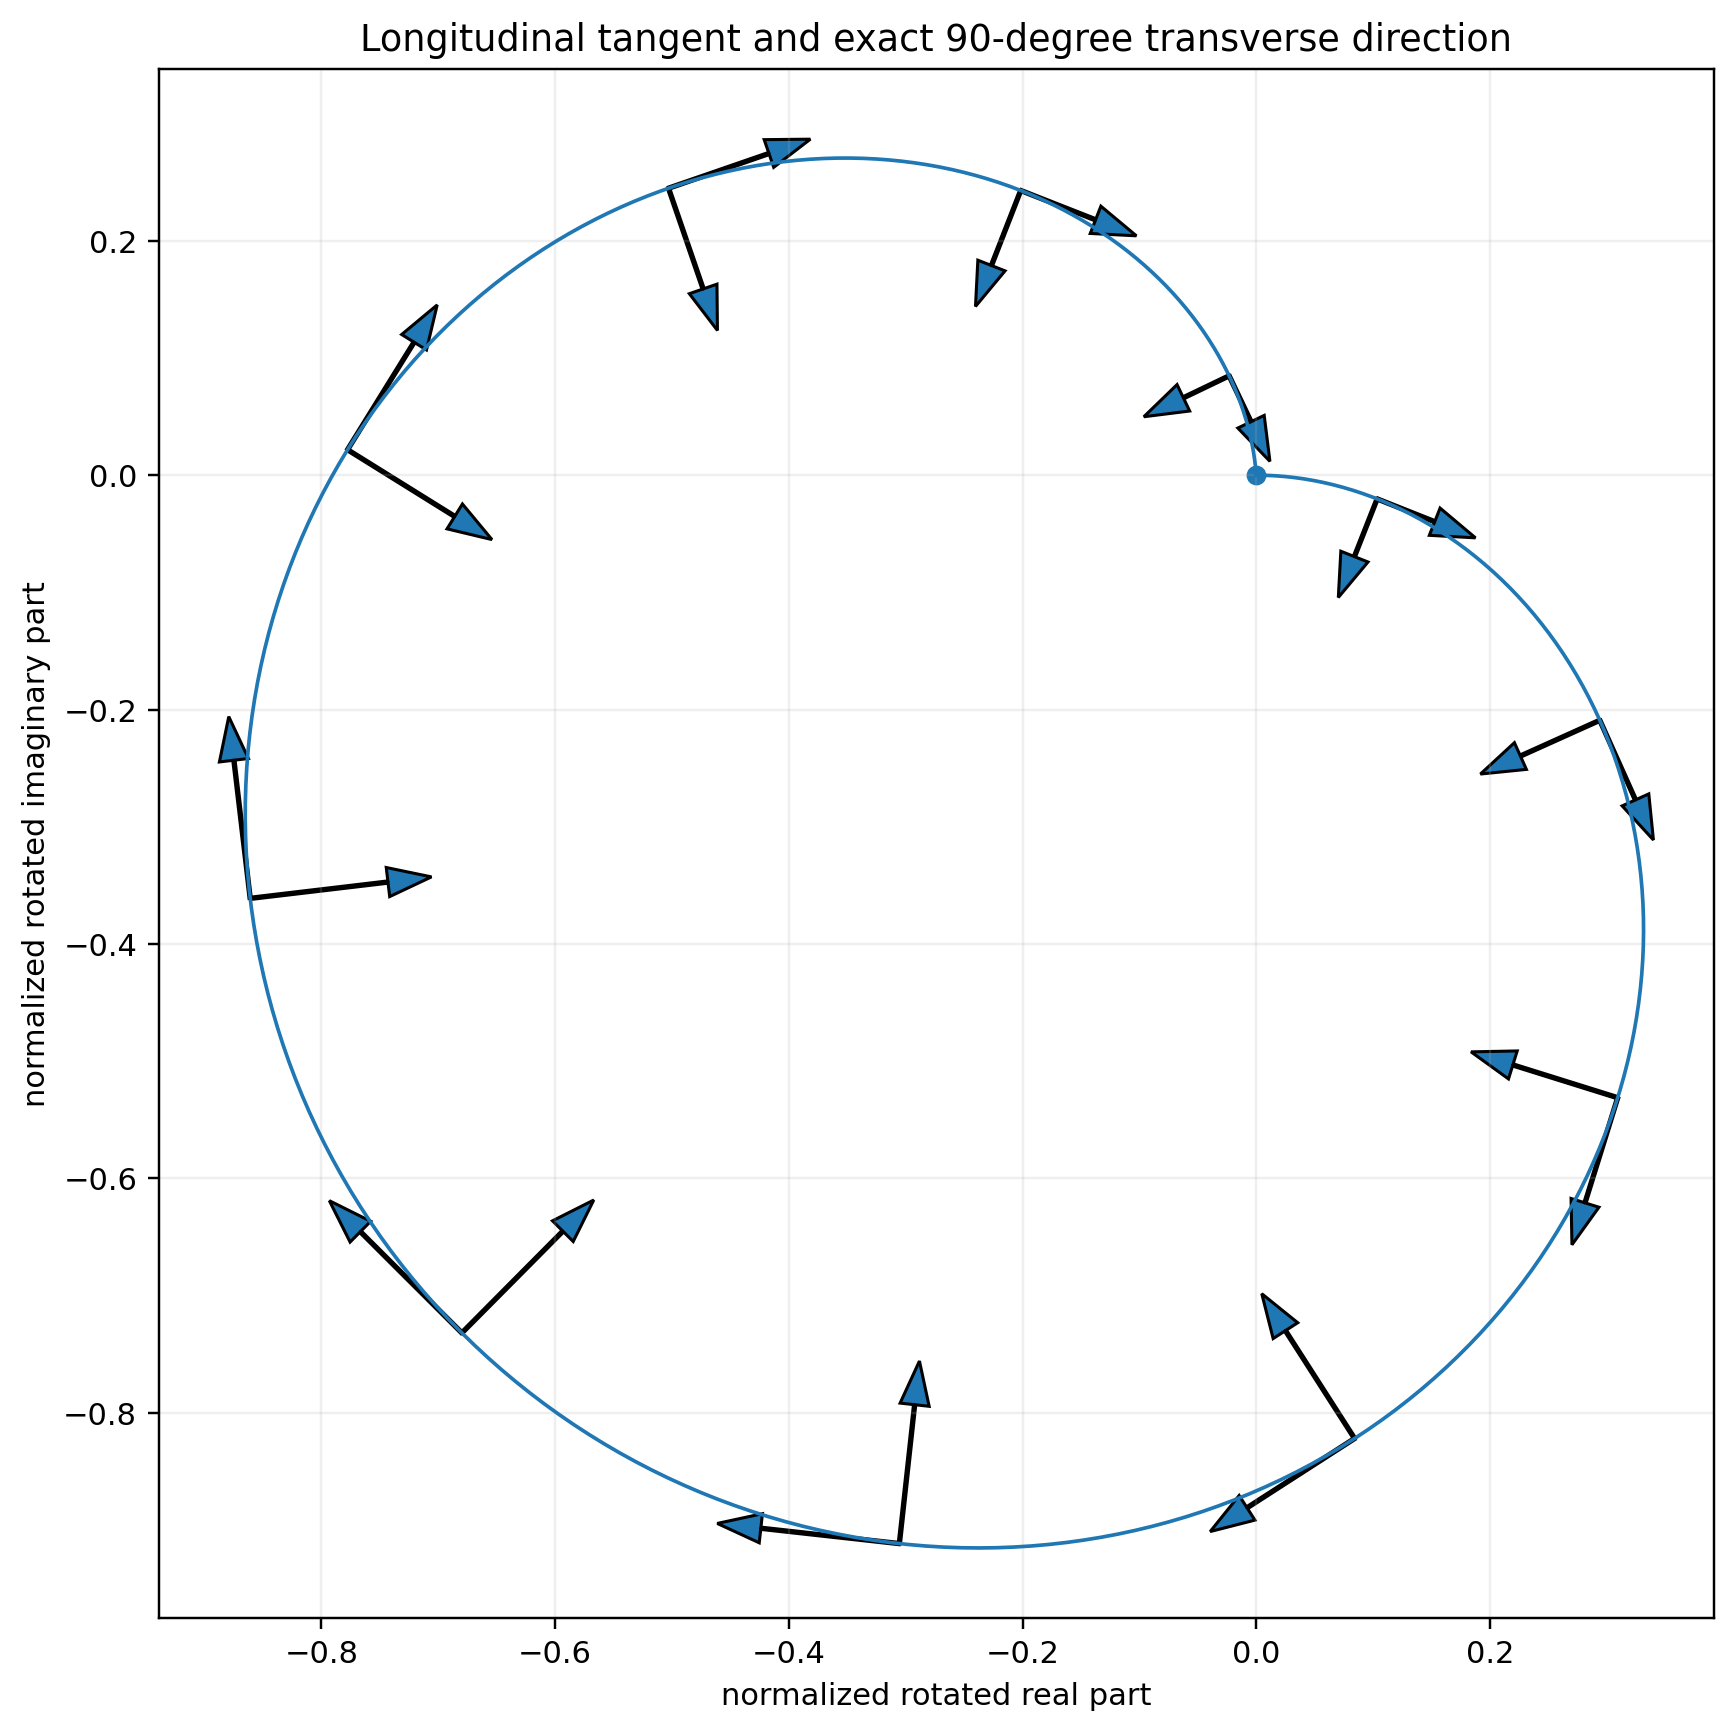
\includegraphics[width=.56\textwidth]{../figures/fig18_quarter_turn_vector_field.png}
\caption{Longitudinal tangent vectors and their exact quarter-turned transverse directions along a representative lobe.}
\label{fig:quarter-turn-vectors}
\end{figure}

\begin{remark}[First order means the complete evolution law]
\label{rem:first-order-complete}
Repeated differentiation of \eqref{eq:quarter-turn} yields identities such as
\begin{equation}
F_{\delta\delta}=-F_{tt},
\qquad
F_{\delta\delta\delta}=iF_{ttt},
\label{eq:higher-derived}
\end{equation}
but these are consequences of the same first-order equation and are not independent dynamical conditions.
\end{remark}

\section{Exact RVM no-exit theorem}
\label{sec:rvm-no-exit}

Analytically continue the RVM skeleton by
\begin{equation}
M(\delta,t)=\frac12\left(1+e^{-2i\Theta_0(t-i\delta)}\right).
\label{eq:M-transverse}
\end{equation}
It satisfies the same quarter-turn equation
\begin{equation}
M_\delta=-iM_t.
\label{eq:M-quarter-turn}
\end{equation}

\begin{theorem}[RVM tangent-circle no-exit]
\label{thm:rvm-no-exit}
For $t>2\pi$ and $\delta\neq0$,
\begin{equation}
M(\delta,t)\neq0.
\label{eq:M-nonzero}
\end{equation}
Moreover,
\begin{equation}
|M(\delta,t)|
\ge
\frac12\left|1-\left(\frac{t}{2\pi}\right)^{-\delta}\right|>0.
\label{eq:M-barrier}
\end{equation}
\end{theorem}

\begin{proof}
Let
\begin{equation}
v(\delta)=\Imm\Theta_0(t-i\delta).
\label{eq:v-definition}
\end{equation}
Since
\begin{equation}
\Theta_0'(z)=\frac12\log\frac{z}{2\pi},
\label{eq:Theta0-prime}
\end{equation}
we obtain
\begin{equation}
v'(\delta)=-\frac12\log\frac{\sqrt{t^2+\delta^2}}{2\pi}.
\label{eq:v-prime}
\end{equation}
For $t>2\pi$, $v'$ is strictly negative and $v(0)=0$, so $v(\delta)$ has the opposite sign to $\delta$.  If $M(\delta,t)=0$, then $e^{-2i\Theta_0(t-i\delta)}=-1$, whose modulus is one.  However,
\begin{equation}
\left|e^{-2i\Theta_0(t-i\delta)}\right|=e^{2v(\delta)}\neq1
\label{eq:RVM-modulus-neq1}
\end{equation}
for $\delta\neq0$, proving \eqref{eq:M-nonzero}.  Finally,
\begin{equation}
|v(\delta)|\ge\frac{|\delta|}{2}\log\frac{t}{2\pi}
\label{eq:v-lower}
\end{equation}
and the reverse triangle inequality applied to \eqref{eq:M-transverse} gives \eqref{eq:M-barrier}.
\end{proof}

\begin{figure}[tbp]
\centering
\begin{subfigure}[t]{.47\textwidth}
\centering
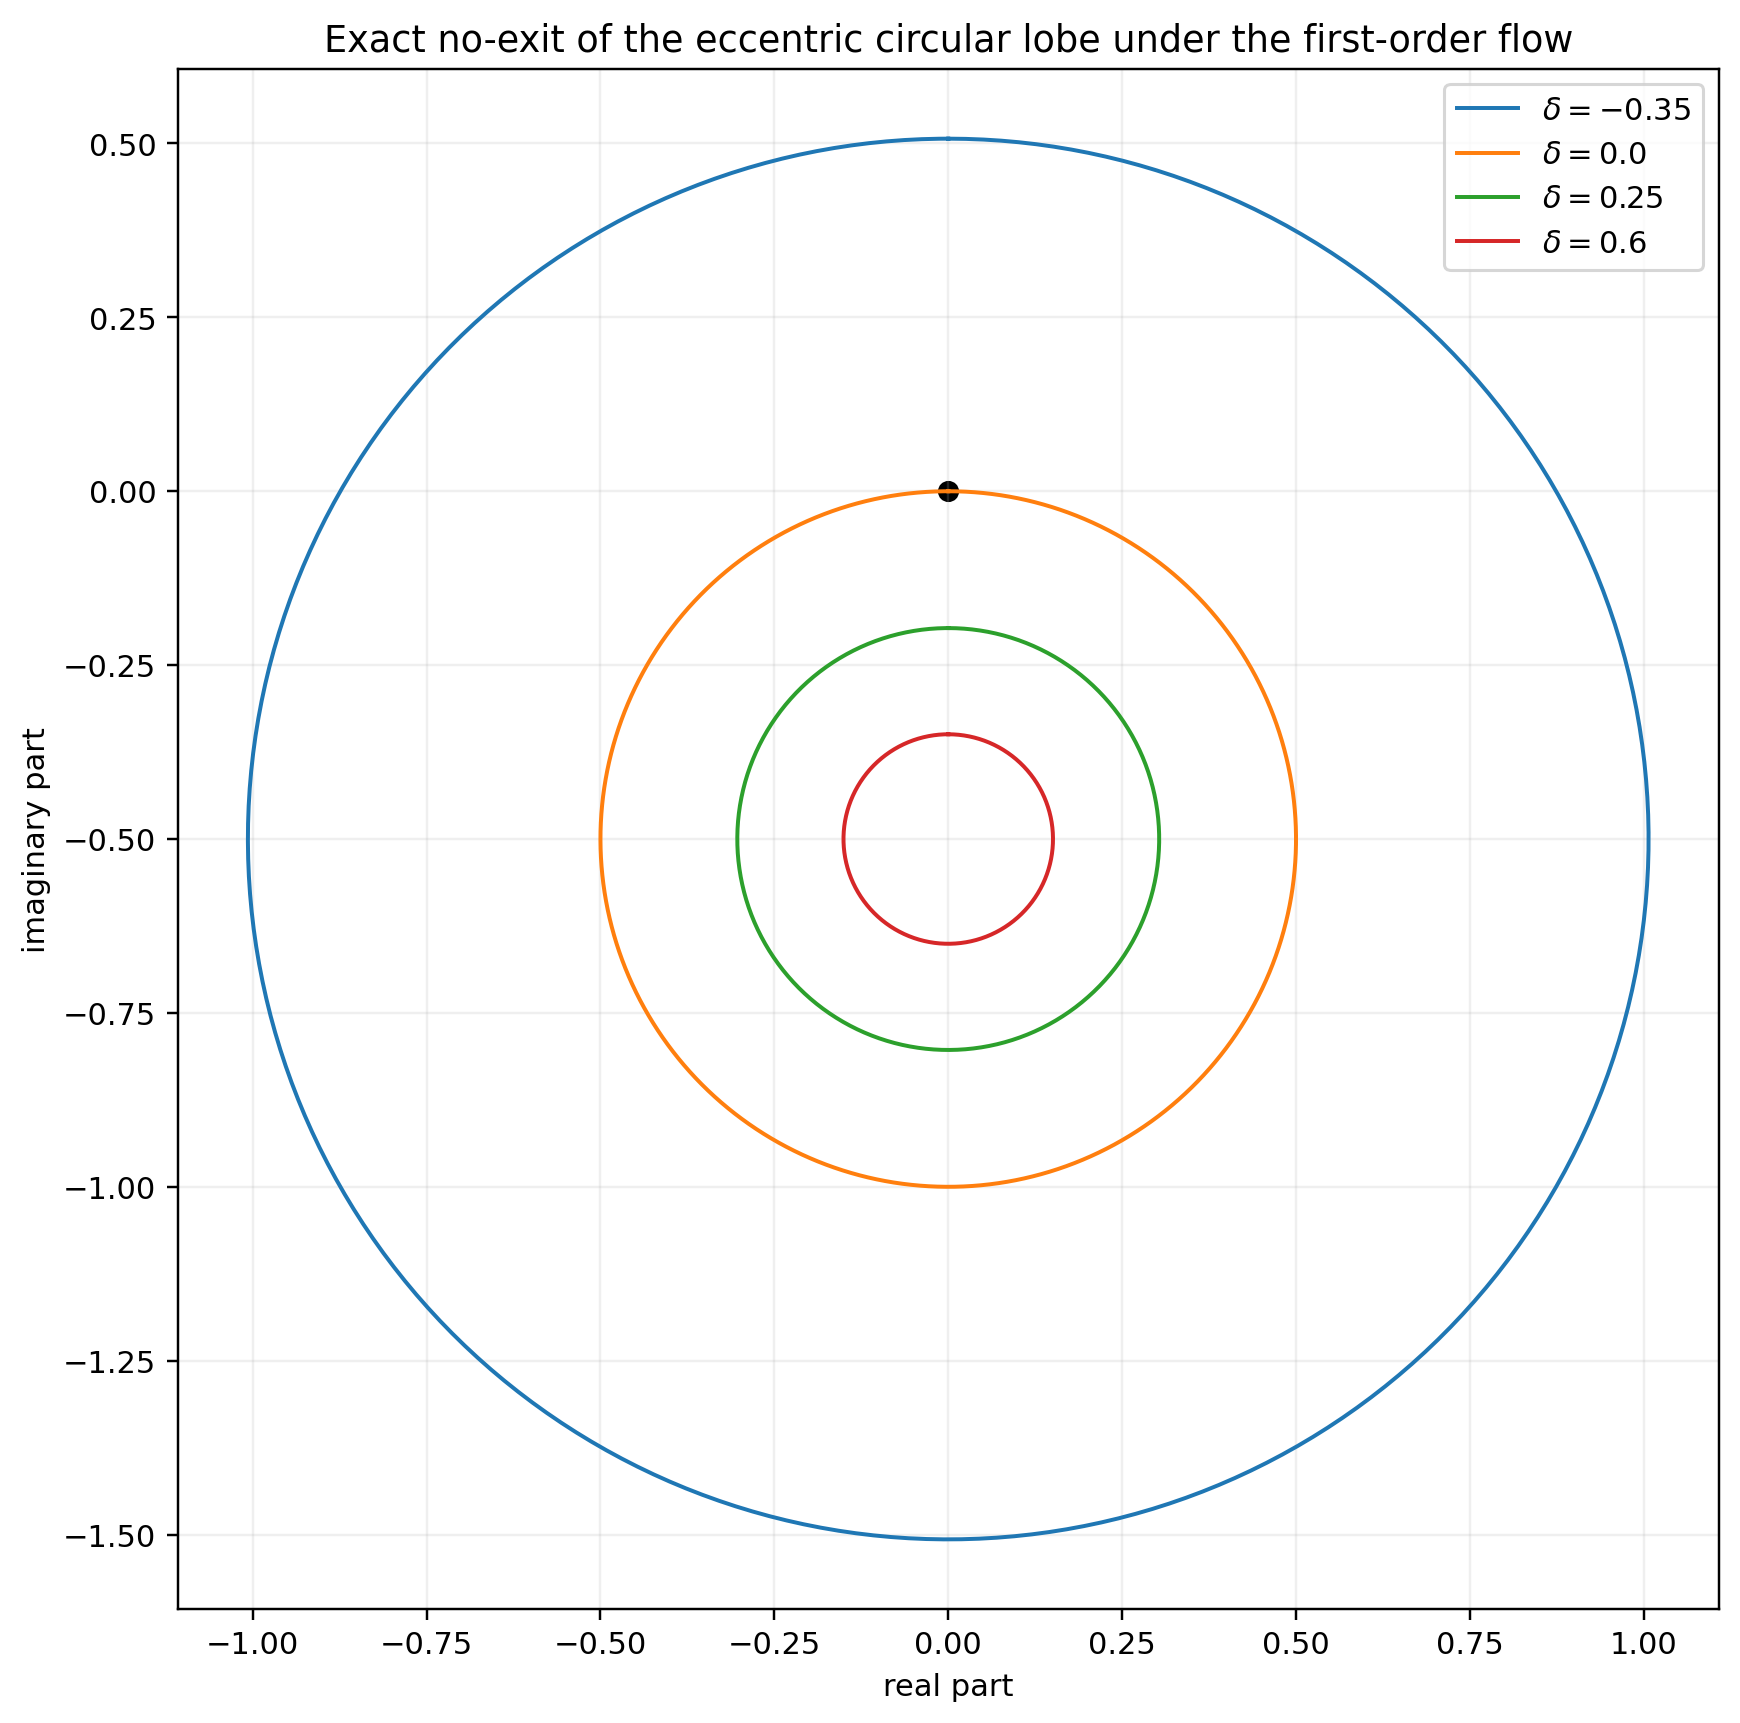
\includegraphics[width=\linewidth]{../figures/fig04_circular_lobe_first_order_no_exit.png}
\caption{Constant-speed circular model.}
\label{fig:circular-no-exit}
\end{subfigure}\hfill
\begin{subfigure}[t]{.47\textwidth}
\centering
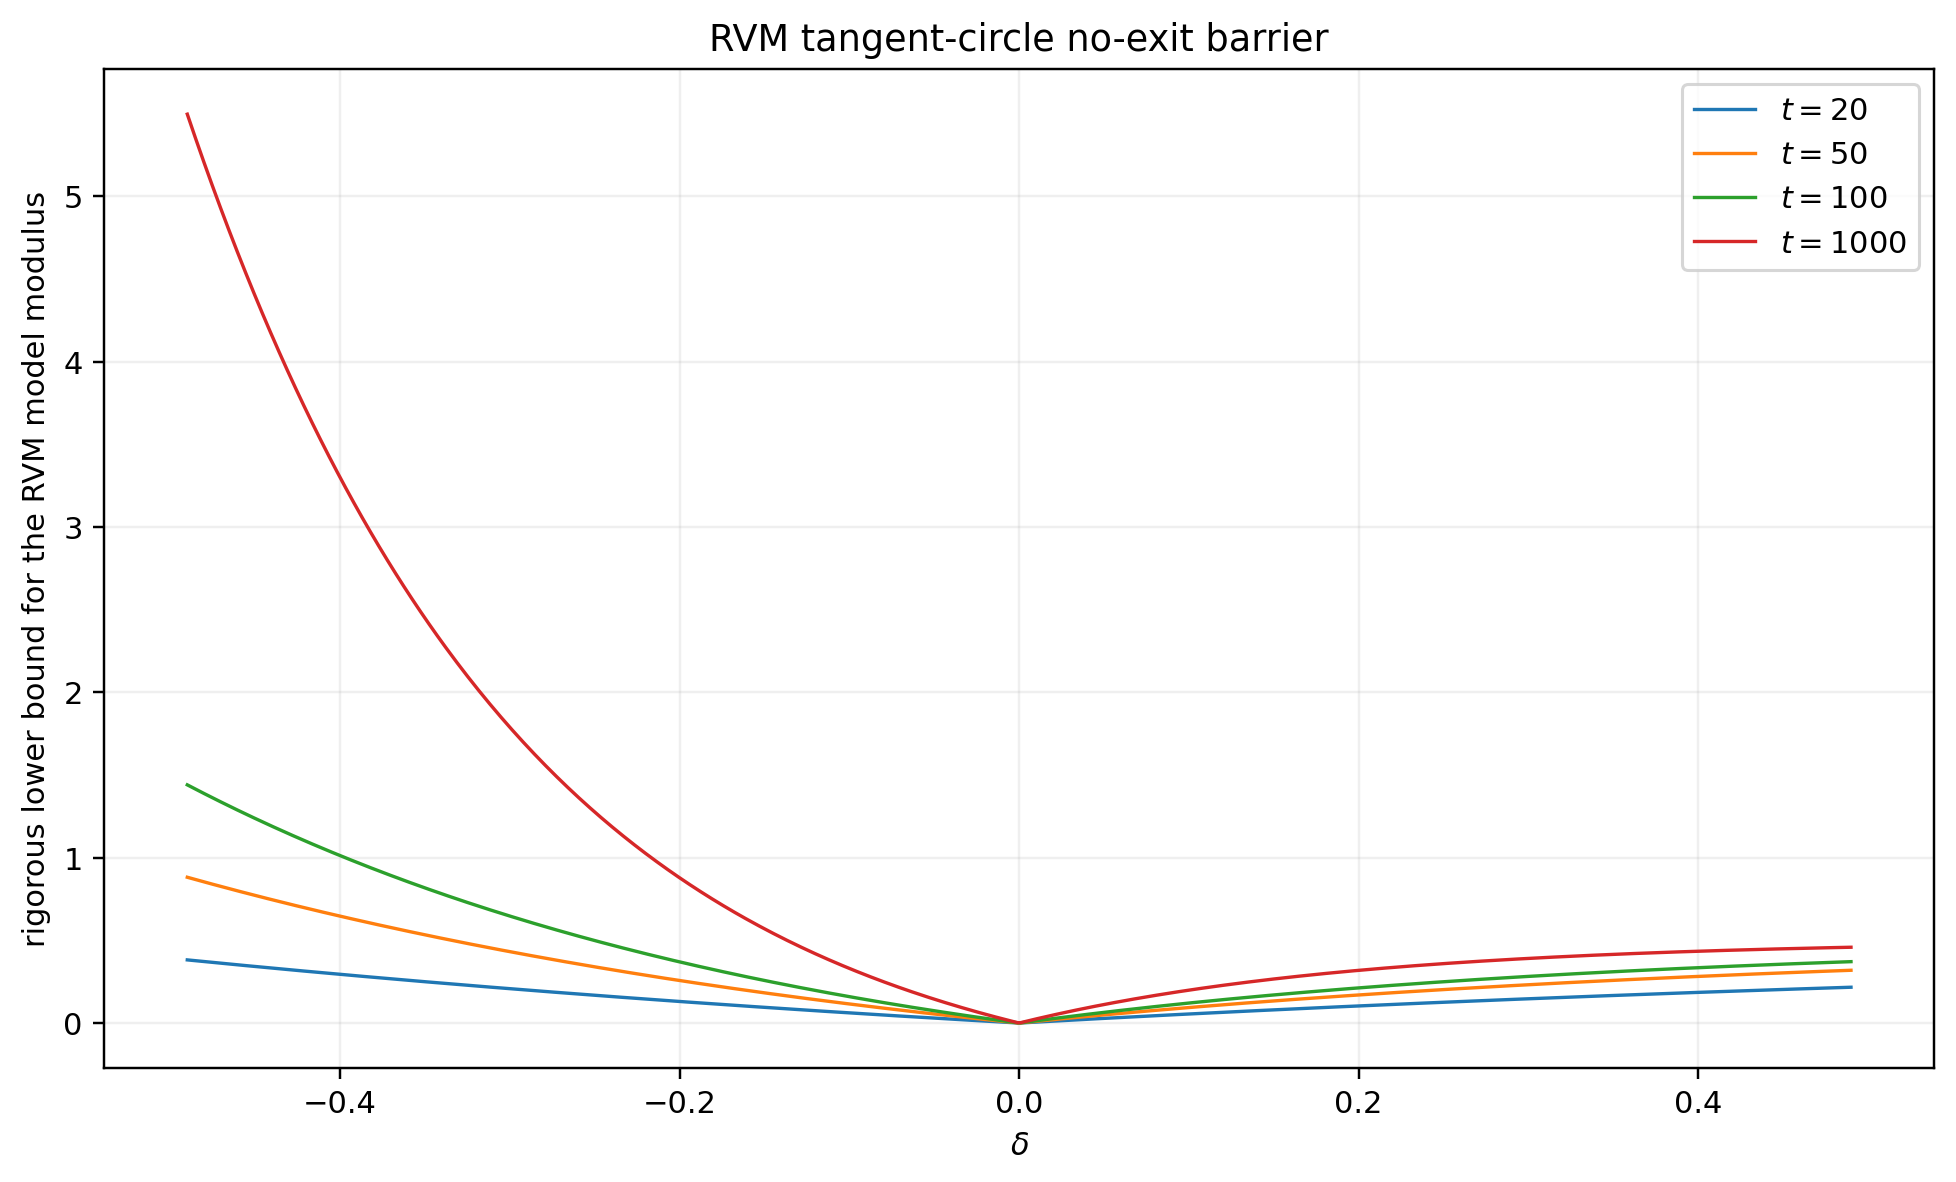
\includegraphics[width=\linewidth]{../figures/fig15_rvm_no_exit_barrier.png}
\caption{Explicit RVM modulus barrier.}
\label{fig:rvm-barrier}
\end{subfigure}
\caption{Two representations of the exact first-order no-exit mechanism in the RVM tangent-circle model.}
\label{fig:rvm-no-exit-pair}
\end{figure}

\section{Reciprocal chart: exact equivalence and actual methodological gain}
\label{sec:reciprocal-equivalence}

Where $F\neq0$, define
\begin{equation}
U(\delta,t)=\frac1{F(\delta,t)}.
\label{eq:U-definition}
\end{equation}

\begin{proposition}[Zero--pole equivalence at the same domain point]
\label{prop:zero-pole-equivalence}
Let $p=(\delta_0,t_0)$ and suppose $F$ is analytic in the corresponding complex domain coordinate.  If $F$ has a zero of order $m$ at $p$, then $U=1/F$ has a pole of order $m$ at the same point, and conversely:
\begin{equation}
\ord_p(U)=-\ord_p(F).
\label{eq:order-reciprocal}
\end{equation}
Thus the statement ``a new pole appears in $U$'' is exactly the statement ``a new zero appears in $F$'' viewed in the reciprocal chart of the Riemann sphere.
\end{proposition}

\begin{proof}
Write
\begin{equation}
F(z)=(z-z_0)^m h(z),
\qquad h(z_0)\neq0.
\label{eq:local-zero-factor}
\end{equation}
Then
\begin{equation}
U(z)=(z-z_0)^{-m}h(z)^{-1},
\label{eq:local-pole-factor}
\end{equation}
which proves \eqref{eq:order-reciprocal}.
\end{proof}

\begin{proposition}[Quarter-turn invariance under inversion]
\label{prop:U-quarter-turn}
On every domain where $U$ is defined,
\begin{equation}
U_\delta=-iU_t.
\label{eq:U-quarter-turn}
\end{equation}
\end{proposition}

\begin{proof}
From \eqref{eq:U-definition} and \eqref{eq:quarter-turn},
\begin{align}
U_\delta
&=-\frac{F_\delta}{F^2}
\label{eq:Udelta-step}\\
&=\frac{iF_t}{F^2}
=-iU_t.
\label{eq:Udelta-final}
\end{align}
\end{proof}

\begin{remark}[Methodological, not logical, change]
\label{rem:reciprocal-method}
On a region $D$ where the reciprocal chart is holomorphic, the inequalities
\begin{equation}
\sup_D|U|\le M
\quad\Longleftrightarrow\quad
\inf_D|F|\ge M^{-1}
\label{eq:upper-lower-equivalence}
\end{equation}
are identical information.  The reciprocal chart can nevertheless alter the available method because upper bounds for holomorphic functions can interact naturally with maximum-modulus and Phragmén--Lindelöf arguments.  Establishing the holomorphy or pole-exclusion required to use those tools is part of the same zero-confinement problem; inversion does not create an independent RH criterion.
\end{remark}

The RVM tangent circle becomes particularly simple under \eqref{eq:U-definition}.  For
\begin{equation}
\widehat W_{\mathrm{RVM}}(\phi)=A\sin\phi\,e^{-i\phi},
\qquad 0<\phi<\pi,
\label{eq:RVM-direct-phi}
\end{equation}
we have
\begin{equation}
U_{\mathrm{RVM}}(\phi)=\frac1A\cot\phi+\frac{i}{A},
\label{eq:RVM-inverse-line}
\end{equation}
which is an exact straight line.  The two zero contacts of the direct lobe become the two infinite ends of the reciprocal branch.

\section{Reciprocal curvature and scattering normal form}
\label{sec:reciprocal-scattering}

Write a rotated lobe as
\begin{equation}
\widehat W_n(\phi)=r_n(\phi)e^{-i\phi},
\qquad 0<\phi<\Omega_n,
\label{eq:lobe-phi}
\end{equation}
and define
\begin{equation}
U_n(\phi)=\frac{e^{i\phi}}{r_n(\phi)}.
\label{eq:Un-phi}
\end{equation}

\begin{proposition}[Reciprocal curvature]
\label{prop:reciprocal-curvature}
The signed curvature of the reciprocal branch has the form
\begin{equation}
\kappa_{U_n}(\phi)
=
\frac{r_n(\phi)^3\bigl(r_n(\phi)+r_n''(\phi)\bigr)}
{\bigl(r_n(\phi)^2+r_n'(\phi)^2\bigr)^{3/2}}.
\label{eq:reciprocal-curvature}
\end{equation}
Hence
\begin{equation}
\sgn\kappa_{U_n}=\sgn\bigl(r_n+r_n''\bigr).
\label{eq:reciprocal-curvature-sign}
\end{equation}
\end{proposition}

\begin{proof}
In polar form the reciprocal radius is $\rho=1/r_n$.  Substitution into the standard polar-curvature expression
\begin{equation}
\kappa=\frac{\rho^2+2\rho'^2-\rho\rho''}{(\rho^2+\rho'^2)^{3/2}}
\label{eq:polar-curvature}
\end{equation}
gives \eqref{eq:reciprocal-curvature}.
\end{proof}

For the one-arch family $r(\phi)=A\sin(\phi/s_n)$,
\begin{equation}
r''(\phi)+r(\phi)=\left(1-\frac1{s_n^2}\right)r(\phi),
\label{eq:arch-curvature-sign}
\end{equation}
so the RVM value $s_n=1$ is precisely the zero-curvature reciprocal state.

Now assume the two endpoint zeros of the lobe are simple and define
\begin{equation}
a_n=\frac{|Z'(\gamma_n)|}{\vartheta'(\gamma_n)},
\qquad
a_{n+1}=\frac{|Z'(\gamma_{n+1})|}{\vartheta'(\gamma_{n+1})}.
\label{eq:a-endpoints}
\end{equation}
The reciprocal asymptotics at the two ends show that the scattering-angle defect is
\begin{equation}
\Delta_n^{\mathrm{sc}}=\Omega_n-\pi=\pi(s_n-1).
\label{eq:scattering-angle-defect}
\end{equation}

In uniform phase coordinate $q=\phi/\Omega_n$, write
\begin{equation}
\widehat W_n(q)
=\sin(\pi q)e^{-i\pi s_nq}H_n(q),
\qquad H_n(q)>0.
\label{eq:H-factorization}
\end{equation}
The endpoint values are
\begin{equation}
H_n(0)=s_na_n,
\qquad
H_n(1)=s_na_{n+1}.
\label{eq:H-endpoints}
\end{equation}
Define the endpoint-normalized interior residual
\begin{equation}
J_n(q)=\frac{H_n(q)}{H_n(0)^{1-q}H_n(1)^q}.
\label{eq:J-definition}
\end{equation}
Then
\begin{equation}
J_n(0)=J_n(1)=1,
\qquad J_n(q)>0\quad(0<q<1),
\label{eq:J-boundary}
\end{equation}
and the exact lobe normal form is
\begin{equation}
\widehat W_n(q)
=s_n\sin(\pi q)e^{-i\pi s_nq}
 a_n^{1-q}a_{n+1}^{q}J_n(q).
\label{eq:exact-lobe-normal-form}
\end{equation}

\begin{proposition}[Integrated reciprocal-curvature budget]
\label{prop:curvature-budget}
Let $\ell_n(q)=\log H_n(q)$ and define
\begin{equation}
V_n(q)=\pi^2s_n^2\frac{r_{\phi\phi}+r}{r}.
\label{eq:Vn-definition}
\end{equation}
Then
\begin{equation}
V_n
=\ell_n''+\ell_n'^2+2\pi\cot(\pi q)\ell_n'+\pi^2(s_n^2-1),
\label{eq:Vn-pointwise}
\end{equation}
and
\begin{equation}
\int_0^1\sin^2(\pi q)V_n(q)\dd q
=
\int_0^1\sin^2(\pi q)\ell_n'(q)^2\dd q
+\frac{\pi^2}{2}(s_n^2-1).
\label{eq:curvature-budget}
\end{equation}
\end{proposition}

\begin{proof}
Substitute $r(q)=\sin(\pi q)H_n(q)$ and $\phi=\pi s_nq$ into \eqref{eq:Vn-definition}.  Multiplication by $\sin^2(\pi q)$ turns the linear derivative terms into
\begin{equation}
\frac{\dd}{\dd q}\left(\sin^2(\pi q)\ell_n'(q)\right),
\label{eq:curvature-total-derivative}
\end{equation}
whose endpoint contribution vanishes, giving \eqref{eq:curvature-budget}.
\end{proof}

\section{Corrected endpoint scattering cocycle}
\label{sec:cocycle}

The endpoint quotient must be fixed before any projective construction is used.

\begin{proposition}[Correct endpoint jet quotient]
\label{prop:endpoint-jet-quotient}
For a sign-normalized lobe
\begin{equation}
w_n(q)=r_n(q)e^{-i\pi s_nq}
\label{eq:wn-q}
\end{equation}
with simple endpoint zeros,
\begin{equation}
w_n'(0)=\pi s_na_n,
\qquad
w_n'(1)=-\pi s_na_{n+1}e^{-i\pi s_n}.
\label{eq:wn-endpoint-derivatives}
\end{equation}
Therefore
\begin{equation}
\Hcal_n:=\frac{w_n'(1)}{w_n'(0)}
=
\frac{a_{n+1}}{a_n}e^{-i(\Omega_n-\pi)}.
\label{eq:Hcal-correct}
\end{equation}
The reciprocal quotient $w_n'(0)/w_n'(1)$ is not the holonomy used below.
\end{proposition}

\begin{proof}
Equation \eqref{eq:H-endpoints} gives
\begin{equation}
r_n'(0)=\pi s_na_n,
\qquad
r_n'(1)=-\pi s_na_{n+1}.
\label{eq:r-endpoint-derivatives}
\end{equation}
At the endpoints the terms proportional to $r_n$ vanish in the derivative of \eqref{eq:wn-q}, yielding \eqref{eq:wn-endpoint-derivatives}.  Since $-e^{-i\pi s_n}=e^{-i\pi(s_n-1)}$, equation \eqref{eq:Hcal-correct} follows.
\end{proof}

Define
\begin{equation}
b_n=\log a_n,
\qquad
\psi_n=\vartheta(\gamma_n)-n\pi.
\label{eq:b-psi}
\end{equation}
Then
\begin{equation}
\psi_{n+1}-\psi_n=\Omega_n-\pi.
\label{eq:psi-increment}
\end{equation}
The corrected complex potential is
\begin{equation}
Q_n=-b_n-i\psi_n.
\label{eq:Q-correct}
\end{equation}
Its conjugate satisfies
\begin{equation}
\overline Q_n-\overline Q_{n+1}
=\log\frac{a_{n+1}}{a_n}-i(\Omega_n-\pi),
\label{eq:Qbar-difference}
\end{equation}
so
\begin{equation}
\Hcal_n=e^{\overline Q_n-\overline Q_{n+1}}.
\label{eq:Hcal-cocycle}
\end{equation}
Equivalently, the oppositely oriented scattering coefficient
\begin{equation}
\mathfrak S_n
=\frac{a_{n+1}}{a_n}e^{i(\Omega_n-\pi)}
=e^{Q_n-Q_{n+1}}
\label{eq:Scattering-cocycle}
\end{equation}
satisfies $\Hcal_n=\overline{\mathfrak S_n}$.

\section{Projective lobe defect: exact identities and corrected branch}
\label{sec:schwarzian}

This section records a projective structure that is exact but is not promoted to a confinement criterion.

\begin{definition}[Schwarzian projective defect]
\label{def:projective-defect}
For a lobe with $w_n'(q)\neq0$, define
\begin{equation}
\{w_n,q\}
=\frac{w_n'''(q)}{w_n'(q)}
-\frac32\left(\frac{w_n''(q)}{w_n'(q)}\right)^2
\label{eq:Schwarzian-definition}
\end{equation}
and
\begin{equation}
\Pcal_n(q)=\{w_n,q\}-2\pi^2.
\label{eq:Pcal-definition}
\end{equation}
\end{definition}

\begin{lemma}[No interior critical point in the lobe parametrization]
\label{lem:no-critical-point}
If $s_n>0$ and $r_n(q)>0$ for $0<q<1$, then
\begin{equation}
w_n'(q)\neq0,
\qquad 0<q<1.
\label{eq:wn-prime-nonzero}
\end{equation}
\end{lemma}

\begin{proof}
From \eqref{eq:wn-q},
\begin{equation}
w_n'(q)=e^{-i\pi s_nq}\left(r_n'(q)-i\pi s_nr_n(q)\right).
\label{eq:wn-prime-factor}
\end{equation}
The bracket has strictly negative imaginary part in the open interval and therefore cannot vanish.
\end{proof}

\begin{theorem}[RVM is the unique positive-sweep constant projective state in the one-arch family]
\label{thm:Schwarzian-arch}
For
\begin{equation}
w_s(q)=A\sin(\pi q)e^{-i\pi sq},
\qquad s>0,
\label{eq:ws-definition}
\end{equation}
the projective defect $\Pcal_s=\{w_s,q\}-2\pi^2$ is
\begin{multline}
\Pcal_s(q)
=-\frac{\pi^2(s^2-1)}{4}
\frac{s^2\cos(2\pi q)-s^2-4is\sin(2\pi q)+3\cos(2\pi q)+9}
{s^2\sin^2(\pi q)+is\sin(2\pi q)-\cos^2(\pi q)}.
\label{eq:Pcal-s-explicit}
\end{multline}
Consequently
\begin{equation}
\Pcal_s\equiv0
\quad\Longleftrightarrow\quad
s=1.
\label{eq:Pcal-s-iff}
\end{equation}
\end{theorem}

\begin{proof}
Direct differentiation of \eqref{eq:ws-definition} gives \eqref{eq:Pcal-s-explicit}.  The factor $s^2-1$ proves one direction.  Conversely, at $q=0$,
\begin{equation}
\Pcal_s(0)=3\pi^2(s^2-1),
\label{eq:Pcal-s-zero}
\end{equation}
so for $s>0$ an identically vanishing defect forces $s=1$.
\end{proof}

Thus the same value $s=1$ is characterized in two independent geometric languages: the direct one-arch lobe is an exact circle by Theorem~\ref{thm:tangent-circle}, and its Schwarzian is exactly the constant $2\pi^2$ by Theorem~\ref{thm:Schwarzian-arch}.

\begin{proposition}[Geometric decomposition of the Schwarzian]
\label{prop:Schwarzian-geometry}
Write
\begin{equation}
w_n'(q)=v(q)e^{i\tau(q)},
\qquad v(q)>0,
\label{eq:tangent-polar}
\end{equation}
and let $\kappa$ be the Euclidean curvature with respect to arc length $s_{\mathrm{arc}}$.  Then
\begin{align}
\Ree\{w_n,q\}
&=(\log v)''-\frac12(\log v)'^2+\frac12\tau'^2,
\label{eq:Schwarzian-real}\\
\Imm\{w_n,q\}
&=\tau''-(\log v)'\tau'
=v^2\frac{\dd\kappa}{\dd s_{\mathrm{arc}}}.
\label{eq:Schwarzian-imag}
\end{align}
\end{proposition}

\begin{proof}
Set $A=w_n''/w_n'=(\log v)'+i\tau'$.  Since
\begin{equation}
\{w_n,q\}=A'-\frac12A^2,
\label{eq:Schwarzian-A}
\end{equation}
the first two expressions follow by taking real and imaginary parts.  Using $\tau'=\kappa v$ converts the imaginary part to the final term in \eqref{eq:Schwarzian-imag}.
\end{proof}

\subsection{Schwarzian equation and closure moment}
\label{subsec:Schwarzian-ode}

Fix the continuous square-root branch determined by $w_n'(0)>0$, and define
\begin{equation}
Y_n(q)=\frac{w_n(q)}{\sqrt{w_n'(q)w_n'(0)}}.
\label{eq:Y-definition}
\end{equation}
Then
\begin{equation}
Y_n(0)=0,
\qquad
Y_n'(0)=1.
\label{eq:Y-initial}
\end{equation}

\begin{theorem}[Exact projective ODE]
\label{thm:projective-ode}
The function $Y_n$ satisfies
\begin{equation}
Y_n''+\left(\pi^2+\frac12\Pcal_n(q)\right)Y_n=0.
\label{eq:Y-ODE}
\end{equation}
\end{theorem}

\begin{proof}
Differentiating $w_n/\sqrt{w_n'}$ gives the classical identity
\begin{equation}
\left(\frac{w_n}{\sqrt{w_n'}}\right)''
+\frac12\{w_n,q\}\frac{w_n}{\sqrt{w_n'}}=0.
\label{eq:Schwarzian-ODE-identity}
\end{equation}
The normalization by the constant $\sqrt{w_n'(0)}$ and definition \eqref{eq:Pcal-definition} give \eqref{eq:Y-ODE}.
\end{proof}

Variation of constants around the RVM free arch gives
\begin{equation}
Y_n(q)
=\frac{\sin(\pi q)}{\pi}
-\frac1{2\pi}\int_0^q\sin\bigl(\pi(q-x)\bigr)\Pcal_n(x)Y_n(x)\dd x.
\label{eq:Y-Duhamel}
\end{equation}
Because $w_n(1)=0$, also $Y_n(1)=0$, and \eqref{eq:Y-Duhamel} at $q=1$ yields the exact closure orthogonality
\begin{equation}
\int_0^1\Pcal_n(x)\sin(\pi x)Y_n(x)\dd x=0.
\label{eq:projective-orthogonality}
\end{equation}

\subsection{Correct endpoint derivative and branch}
\label{subsec:Y-endpoint}

The endpoint derivative is the place where the reciprocal error must be excluded.

\begin{proposition}[Correct $Y_n'(1)$ quotient]
\label{prop:Y-endpoint-correct}
With the normalization \eqref{eq:Y-definition},
\begin{equation}
\bigl(Y_n'(1)\bigr)^2
=\frac{w_n'(1)}{w_n'(0)}
=\Hcal_n,
\label{eq:Yprime-square-correct}
\end{equation}
not the reciprocal quotient.
\end{proposition}

\begin{proof}
At $q=1$ the terms proportional to $w_n(1)$ vanish after differentiating \eqref{eq:Y-definition}, so
\begin{equation}
Y_n'(1)=\frac{w_n'(1)}{\sqrt{w_n'(1)w_n'(0)}}.
\label{eq:Yprime1-direct}
\end{equation}
Squaring gives \eqref{eq:Yprime-square-correct}.
\end{proof}

The square root is fixed by the lobe geometry rather than by an arbitrary principal-branch convention.  The factor
\begin{equation}
D_n(q)=r_n'(q)-i\pi s_nr_n(q)
\label{eq:Dfactor-definition}
\end{equation}
lies in the open lower half-plane for $0<q<1$, begins on the positive real axis, and ends on the negative real axis.  Its continuous argument therefore changes by $-\pi$.  Together with $e^{-i\pi s_nq}$ in \eqref{eq:wn-prime-factor},
\begin{equation}
\Delta\arg w_n'=-\pi(s_n+1).
\label{eq:wprime-argument-change}
\end{equation}
Hence the continuously transported square root gives
\begin{equation}
Y_n'(1)
=-\sqrt{\frac{a_{n+1}}{a_n}}
 e^{-\frac{i}{2}(\Omega_n-\pi)}.
\label{eq:Yprime1-correct}
\end{equation}
Define
\begin{equation}
\lambda_n=-Y_n'(1)
=\sqrt{\frac{a_{n+1}}{a_n}}
 e^{-\frac{i}{2}(\Omega_n-\pi)}.
\label{eq:lambda-correct}
\end{equation}
Then
\begin{equation}
\lambda_n^2=\Hcal_n.
\label{eq:lambda-square}
\end{equation}
For the exact RVM lobe, $a_{n+1}=a_n$ and $s_n=1$, so $Y_n'(1)=-1$ and $\lambda_n=1$.

\subsection{Correct complex moment and telescoping law}
\label{subsec:moment-cocycle}

Differentiating \eqref{eq:Y-Duhamel} and setting $q=1$ gives
\begin{equation}
Y_n'(1)
=-1+\frac12\int_0^1\cos(\pi x)\Pcal_n(x)Y_n(x)\dd x.
\label{eq:Yprime-Duhamel}
\end{equation}
Using \eqref{eq:projective-orthogonality} and \eqref{eq:lambda-correct}, define
\begin{equation}
\Ical_n
:=\int_0^1\Pcal_n(x)e^{i\pi x}Y_n(x)\dd x.
\label{eq:Ical-definition}
\end{equation}
Then
\begin{equation}
\Ical_n=2(1-\lambda_n).
\label{eq:Ical-lambda}
\end{equation}
By \eqref{eq:Hcal-cocycle} and the geometrically fixed square-root branch,
\begin{equation}
\lambda_n
=e^{(\overline Q_n-\overline Q_{n+1})/2}.
\label{eq:lambda-Q}
\end{equation}
Therefore, for every $k\ge1$ for which the lobe chain satisfies the stated simplicity assumptions,
\begin{equation}
\prod_{j=n}^{n+k-1}\left(1-\frac{\Ical_j}{2}\right)
=
\exp\left(\frac{\overline Q_n-\overline Q_{n+k}}{2}\right).
\label{eq:projective-product}
\end{equation}

\begin{remark}[What the Schwarzian block does and does not add]
\label{rem:Schwarzian-status}
Equations \eqref{eq:projective-orthogonality}, \eqref{eq:Ical-lambda}, and \eqref{eq:projective-product} are exact.  They reconstruct endpoint scattering from an interior projective defect.  At present they provide no sign, sector, monotonicity, or norm constraint on $\Ical_n$ that would imply \eqref{eq:global-no-exit}.  The projective block is therefore a structural identity layer, not the missing confinement theorem.
\end{remark}

\section{Euclidean arc length and phase-coordinate geometry}
\label{sec:arc-length}

The Euclidean length of the $n$th lobe is
\begin{equation}
L_n
=\int_{\gamma_n}^{\gamma_{n+1}}
\sqrt{1+\left|\zeta'\!\left(\frac12+it\right)\right|^2}\dd t.
\label{eq:Ln-definition}
\end{equation}
Using \eqref{eq:speed-Hardy},
\begin{equation}
L_n
=\int_{\gamma_n}^{\gamma_{n+1}}
\sqrt{1+Z'(t)^2+\vartheta'(t)^2Z(t)^2}\dd t.
\label{eq:Ln-Hardy}
\end{equation}
Define
\begin{equation}
R_n=\frac{L_n}{g_n}.
\label{eq:Rn-definition}
\end{equation}

Let
\begin{equation}
q_\vartheta(t)=\frac{\vartheta(t)}{\pi}.
\label{eq:qtheta}
\end{equation}
Then
\begin{equation}
\dd q_\vartheta=\frac{\vartheta'(t)}{\pi}\dd t,
\label{eq:dqtheta}
\end{equation}
and, writing $r(q_\vartheta)=|Z(t(q_\vartheta))|$,
\begin{equation}
L_n
=\int_{q_n}^{q_{n+1}}
\sqrt{
\left(\frac{\pi}{\vartheta'(t(q_\vartheta))}\right)^2
+\left(\frac{\dd r}{\dd q_\vartheta}\right)^2
+\pi^2r(q_\vartheta)^2
}\dd q_\vartheta.
\label{eq:Ln-phase-coordinate}
\end{equation}
The integration-domain length is exactly
\begin{equation}
q_{n+1}-q_n=s_n.
\label{eq:q-domain-sn}
\end{equation}
Thus the local spacing variable is the phase-coordinate width of the Euclidean lobe itself.  Montgomery's pair-correlation problem \cite{Montgomery1973} concerns a different, all-pairs statistic; the identification in \eqref{eq:q-domain-sn} is specifically a nearest-neighbor geometric statement.

For the one-arch approximation
\begin{equation}
Z(t)\approx A_n\sin\left(\pi\frac{t-\gamma_n}{g_n}\right)
\label{eq:Z-one-arch}
\end{equation}
and locally frozen $\vartheta'$, set
\begin{equation}
a_n^{\mathrm{arc}}=\frac{\pi A_n}{g_n},
\qquad
b_n^{\mathrm{arc}}=A_n\vartheta'(m_n),
\qquad
m_n=\frac{\gamma_n+\gamma_{n+1}}2.
\label{eq:arc-ab}
\end{equation}
Then
\begin{equation}
R_n^{\mathrm{arch}}
=\frac2\pi\sqrt{1+(a_n^{\mathrm{arc}})^2}\,
E\!\left(
\frac{(a_n^{\mathrm{arc}})^2-(b_n^{\mathrm{arc}})^2}
{1+(a_n^{\mathrm{arc}})^2}
\right),
\label{eq:Rn-elliptic}
\end{equation}
where $E$ is the complete elliptic integral of the second kind.

\begin{figure}[tbp]
\centering
\begin{subfigure}[t]{.47\textwidth}
\centering
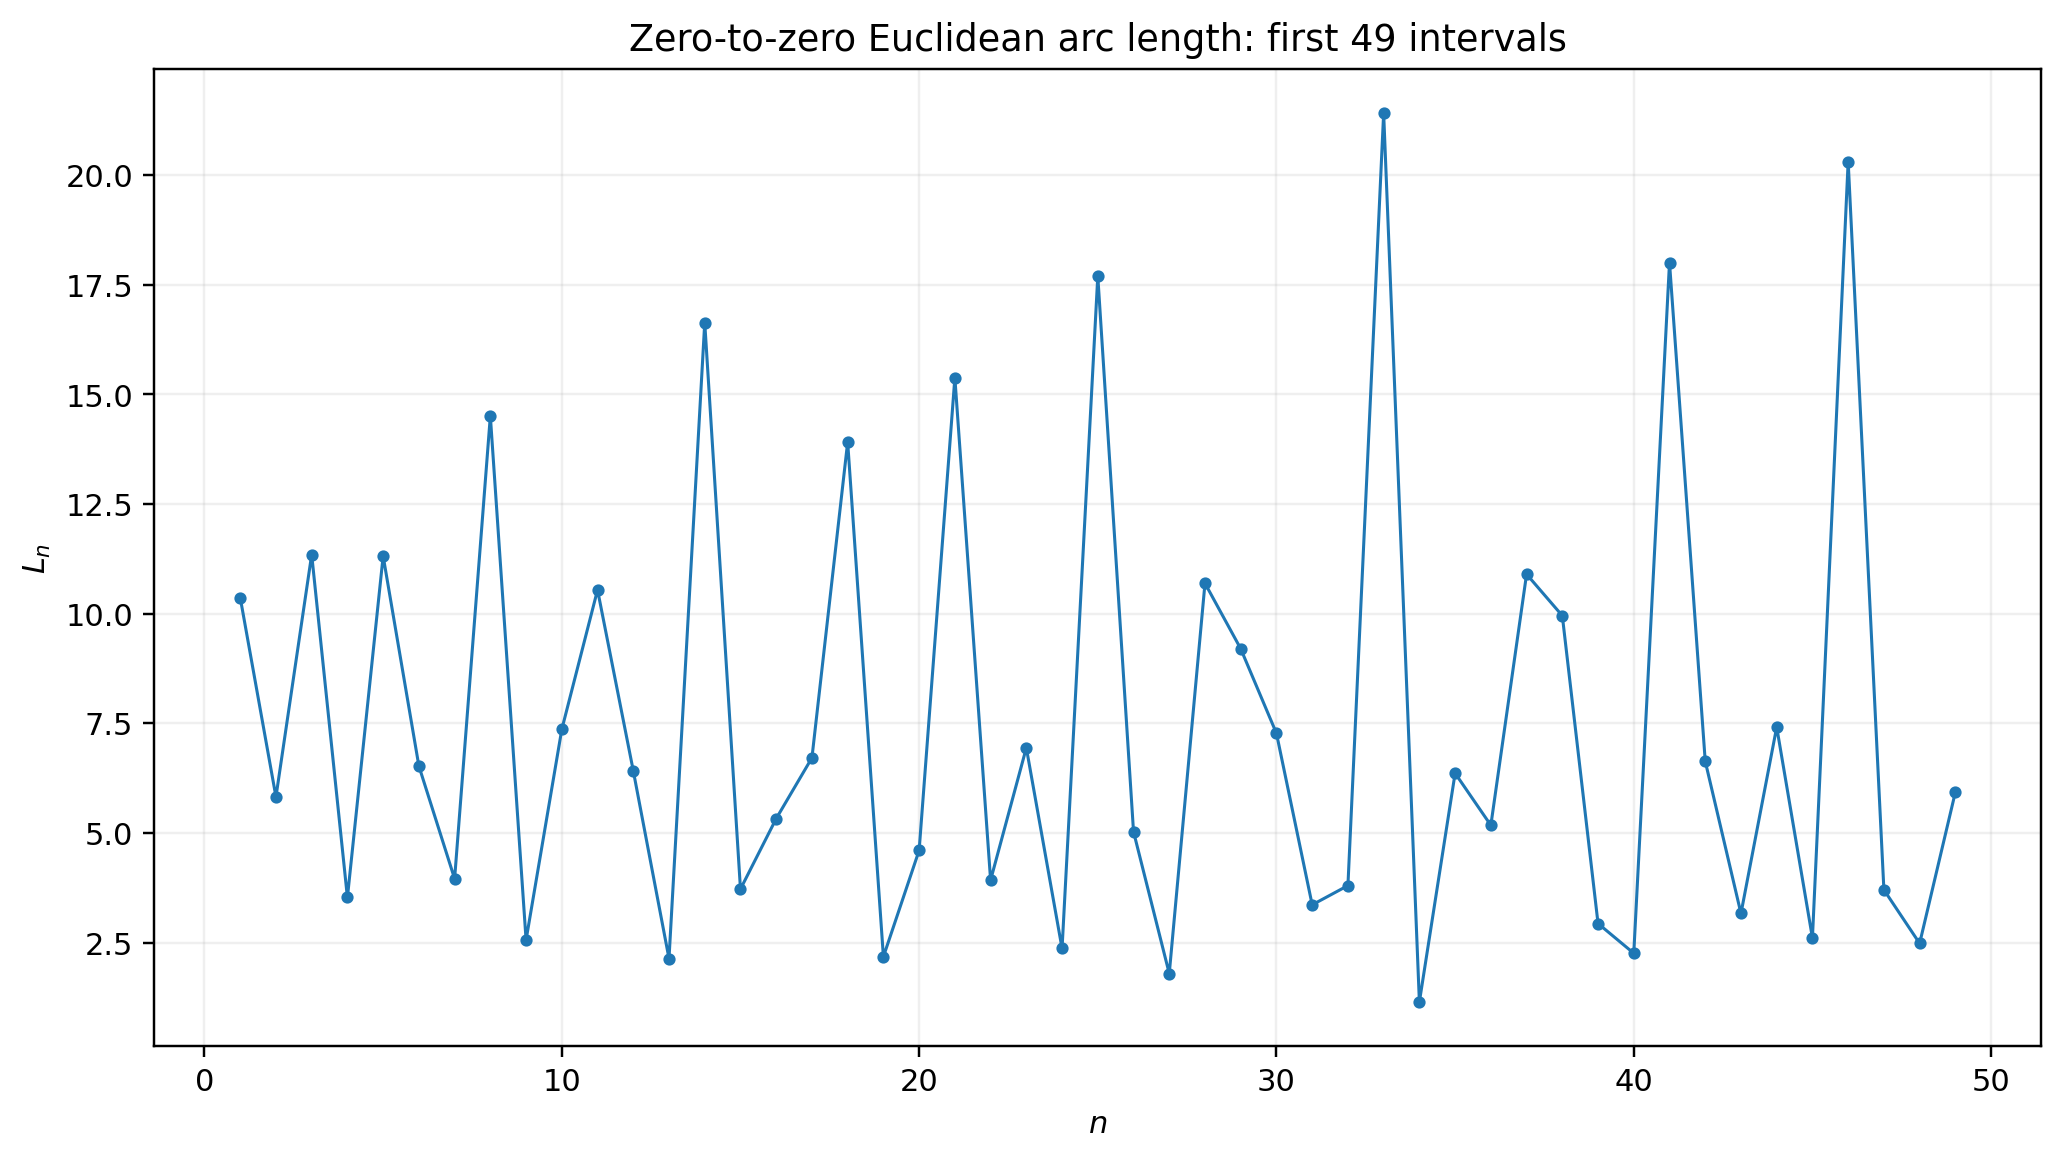
\includegraphics[width=\linewidth]{../figures/fig10_arc_length_Ln.png}
\caption{Euclidean lobe lengths $L_n$.}
\label{fig:Ln}
\end{subfigure}\hfill
\begin{subfigure}[t]{.47\textwidth}
\centering
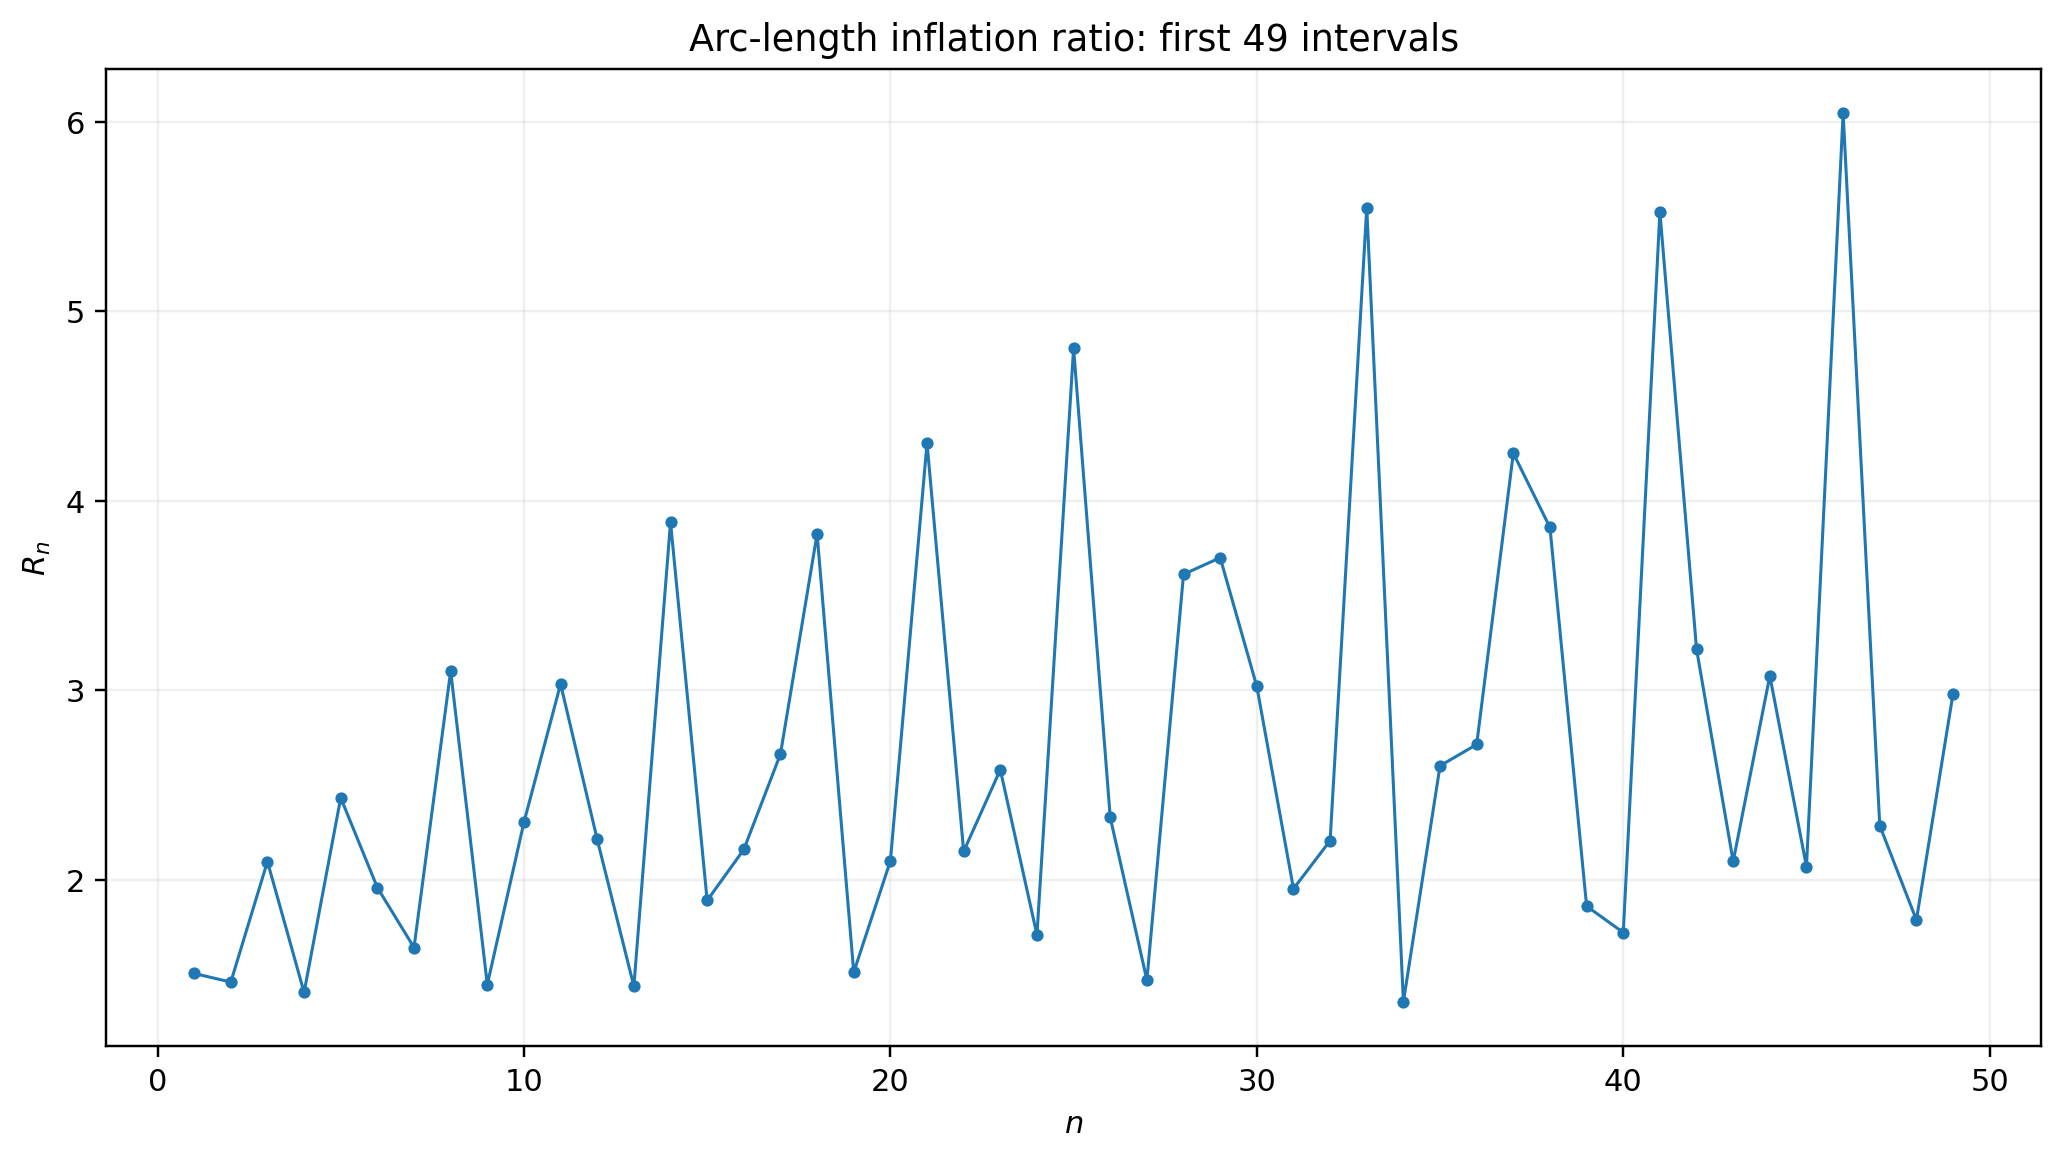
\includegraphics[width=\linewidth]{../figures/fig11_arc_ratio_Rn.png}
\caption{Arc inflation ratios $R_n$.}
\label{fig:Rn}
\end{subfigure}
\caption{Zero-to-zero Euclidean arc geometry for the carried first-49 computation.}
\label{fig:arc-pair}
\end{figure}

\begin{figure}[tbp]
\centering
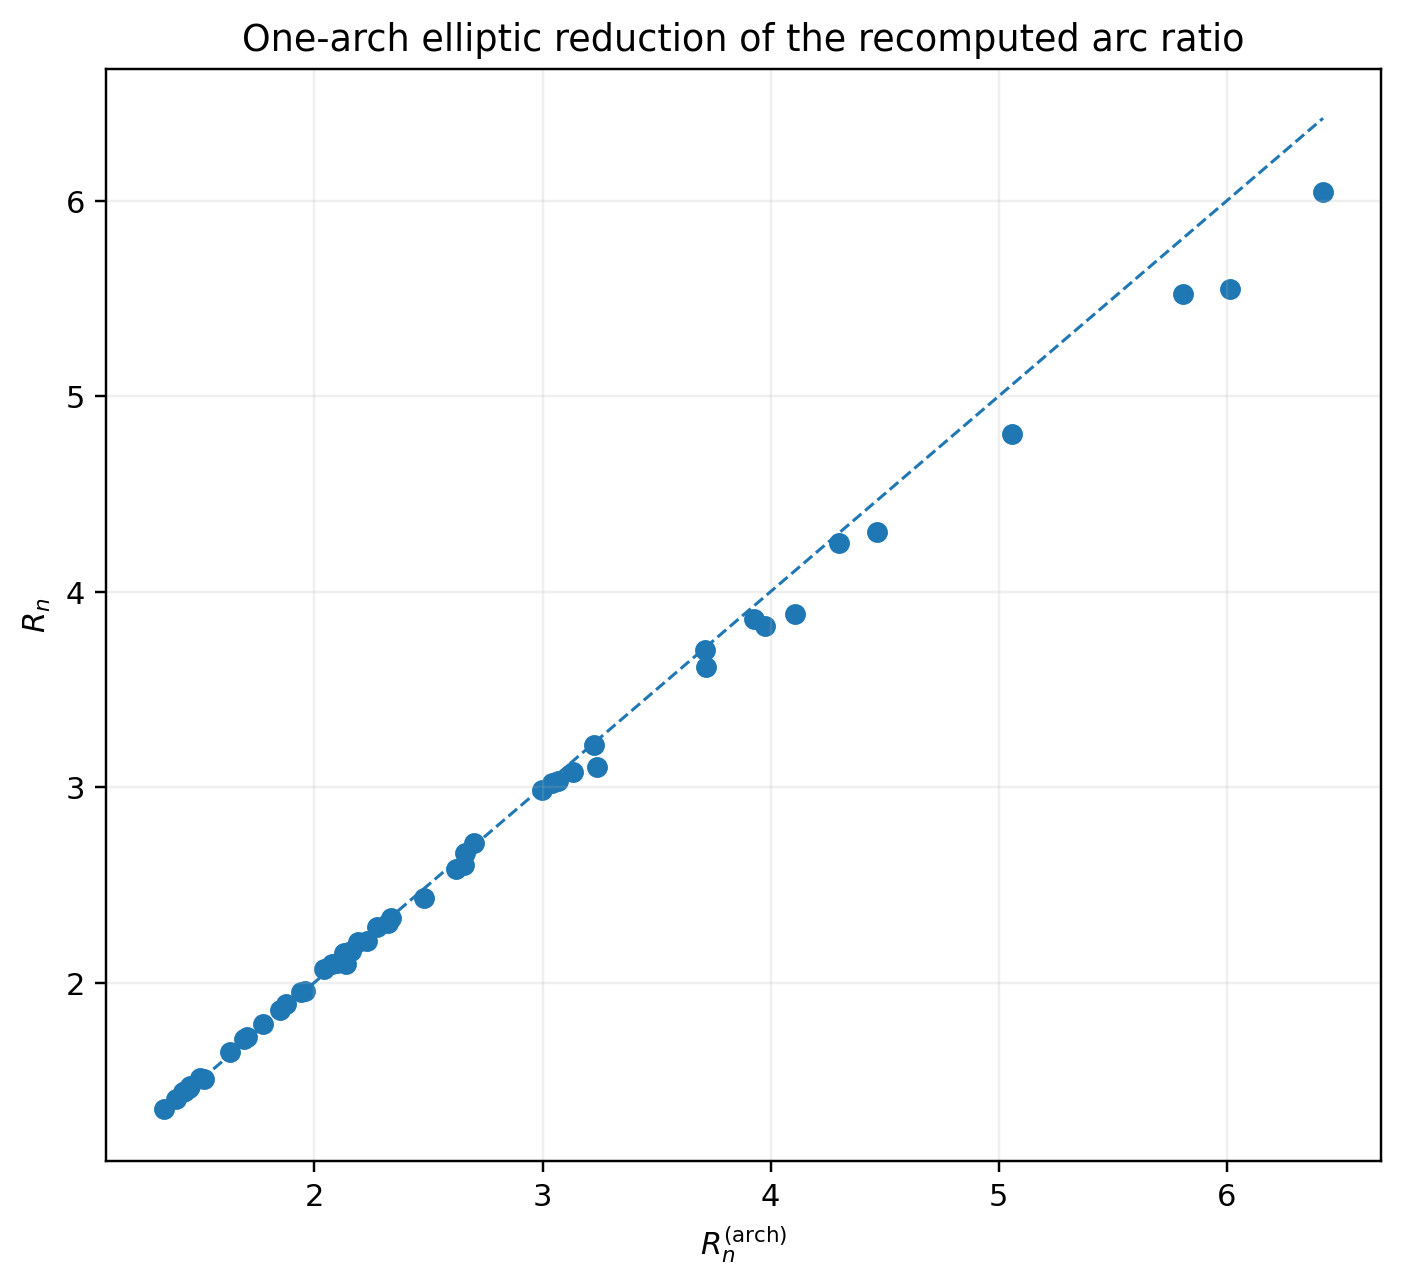
\includegraphics[width=.56\textwidth]{../figures/fig12_elliptic_arch_prediction.png}
\caption{Measured arc inflation versus the one-arch elliptic reduction.}
\label{fig:elliptic-arch}
\end{figure}

\section{Eccentricity observables carried from the preceding computation}
\label{sec:eccentricity-numerics}

For a rotated lobe in uniform phase coordinate define
\begin{equation}
\Ccal_n=\int_0^1\widehat W_n(q)\dd q,
\label{eq:Ccal-definition}
\end{equation}
\begin{equation}
E_n=\frac{2|\Ccal_n|}{A_n},
\label{eq:En-definition}
\end{equation}
and
\begin{equation}
D_n=\frac1{A_n}
\left[
\int_0^1
\left(|\widehat W_n(q)-\Ccal_n|-|\Ccal_n|\right)^2\dd q
\right]^{1/2}.
\label{eq:Dn-definition}
\end{equation}
For the one-arch phase model,
\begin{equation}
\frac{\Ccal_n^{\mathrm{arch}}}{A_n}
=\frac{1+e^{-i\pi s_n}}{\pi(1-s_n^2)},
\label{eq:Ccal-arch}
\end{equation}
with continuous value $-i/2$ at $s_n=1$, and therefore
\begin{equation}
E_n^{\mathrm{arch}}
=\frac{4|\cos(\pi s_n/2)|}{\pi|1-s_n^2|}.
\label{eq:En-arch}
\end{equation}

The carried first-49 values give
\begin{equation}
\operatorname{corr}(E_n,E_n^{\mathrm{arch}})=0.997589,
\qquad
\operatorname{RMSE}=0.017527,
\qquad
\operatorname{MAE}=0.014155,
\label{eq:eccentricity-fit}
\end{equation}
and the carried arc computation gives
\begin{equation}
\operatorname{corr}(R_n,R_n^{\mathrm{arch}})=0.999162,
\qquad
\operatorname{RMSE}=0.116004.
\label{eq:arc-fit}
\end{equation}
These are numerical statements, not analytic hypotheses used in the exact theorems above.

\begin{figure}[tbp]
\centering
\begin{subfigure}[t]{.47\textwidth}
\centering
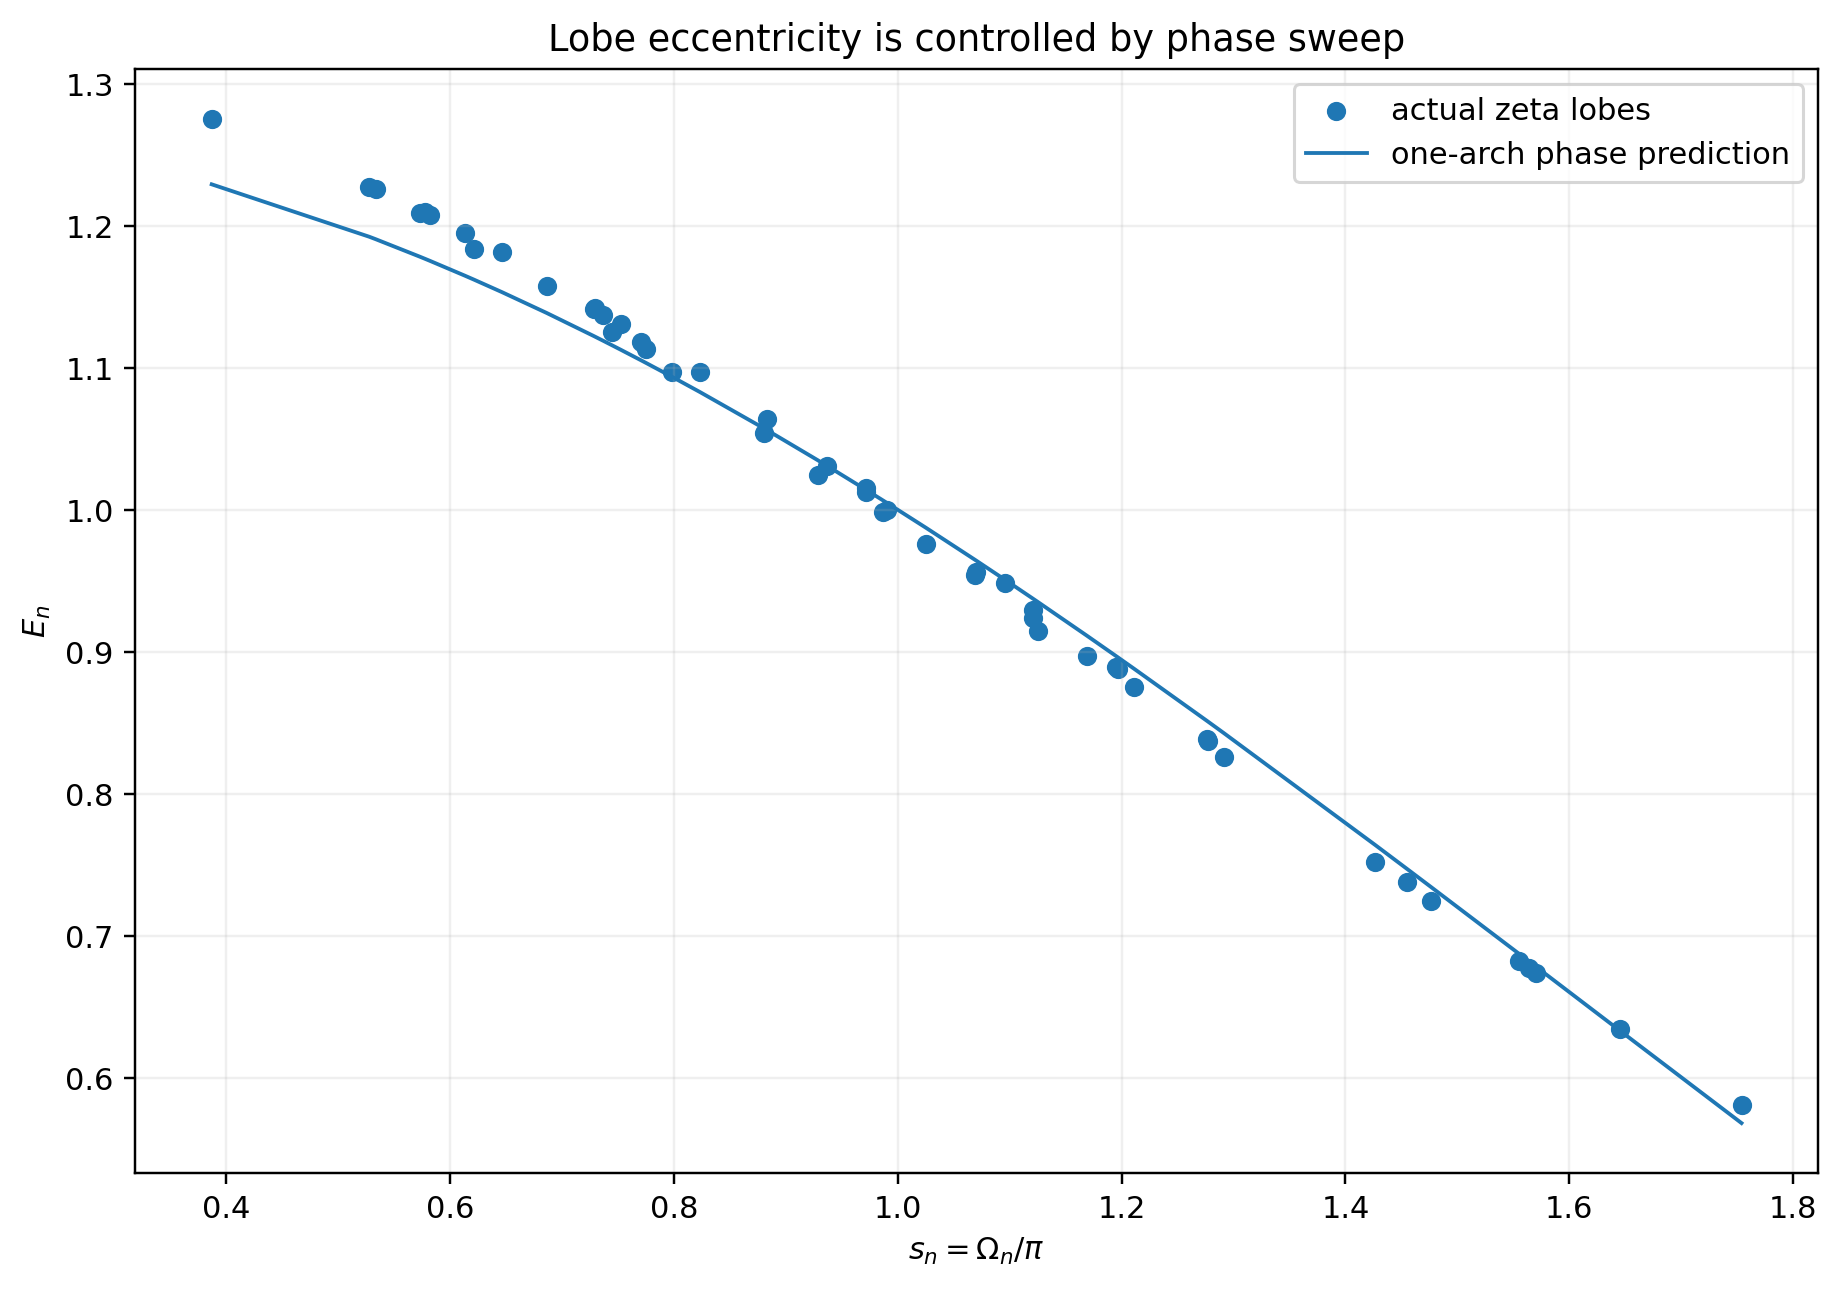
\includegraphics[width=\linewidth]{../figures/fig19_eccentricity_phase_law.png}
\caption{Eccentricity versus phase sweep.}
\label{fig:eccentricity-phase-law}
\end{subfigure}\hfill
\begin{subfigure}[t]{.47\textwidth}
\centering
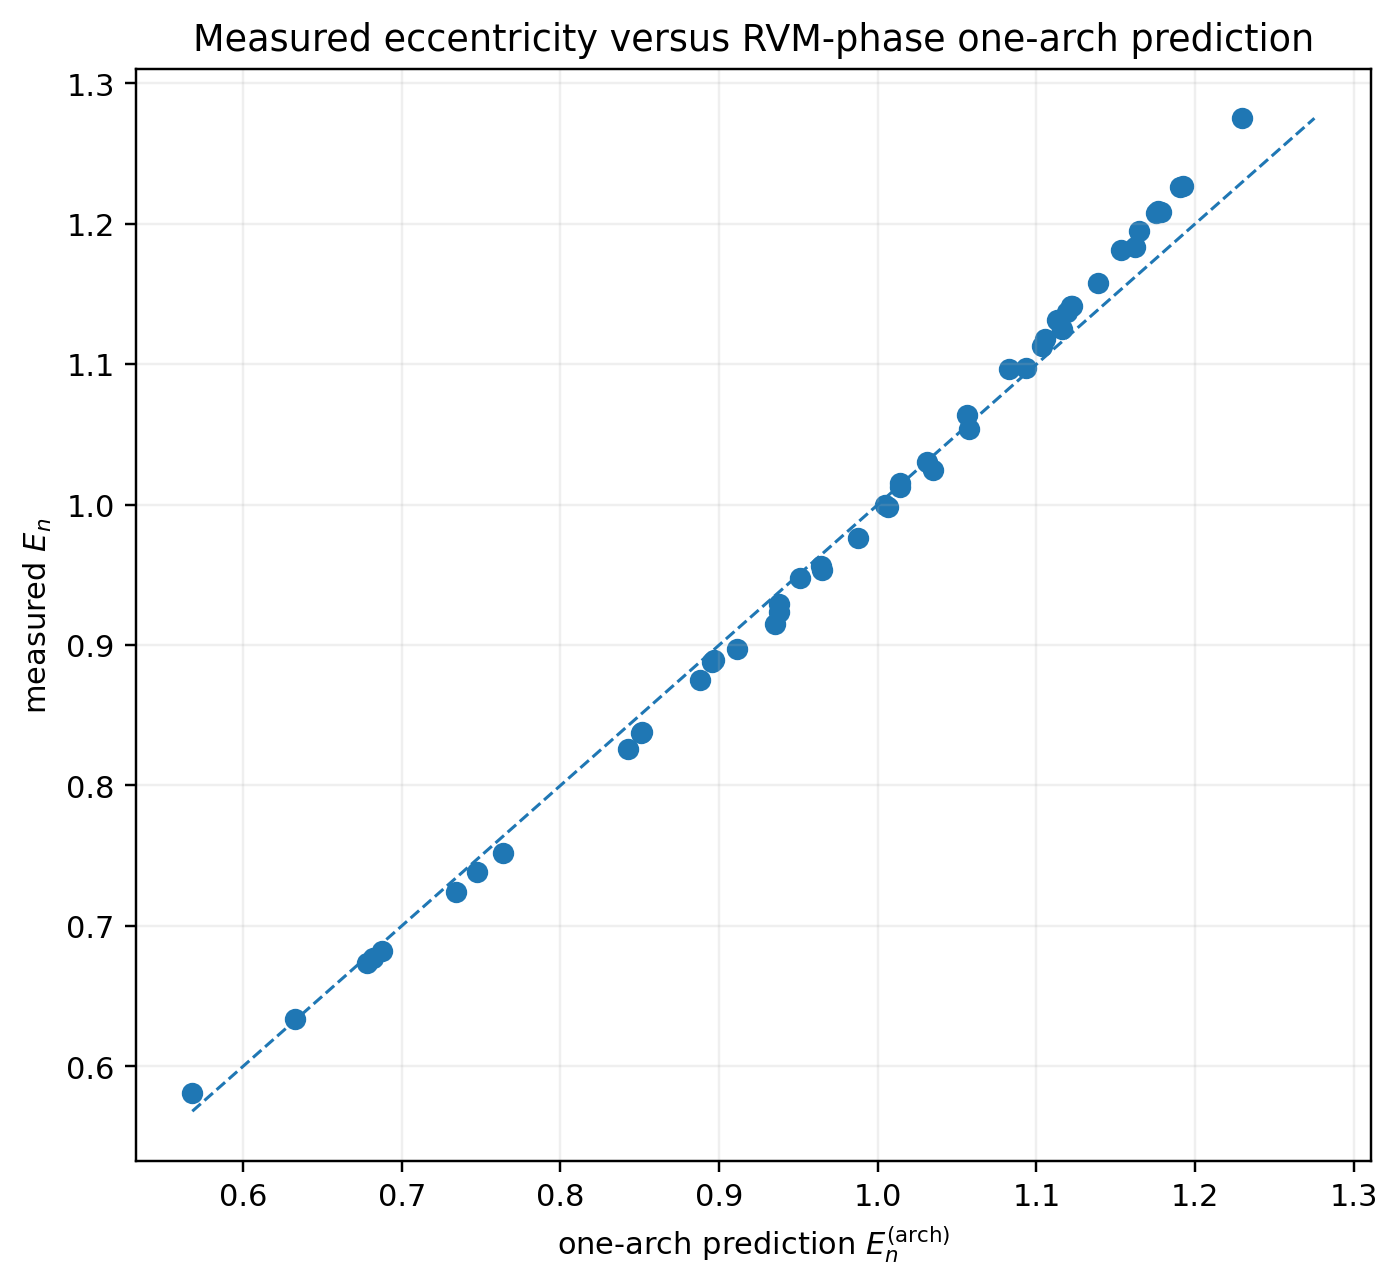
\includegraphics[width=\linewidth]{../figures/fig14_eccentricity_model_vs_actual.png}
\caption{Measured versus one-arch eccentricity.}
\label{fig:eccentricity-fit}
\end{subfigure}
\caption{The carried numerical eccentricity diagnostics.}
\label{fig:eccentricity-pair}
\end{figure}

\section{Full carried phase/RVM audit}
\label{sec:full-audit}

The package carries the previously verified $2{,}001{,}052$ zeta ordinates and the same number of RVM/Lambert ordinates.  Version 5 does not inspect or recompute those binary files.  The preceding audit reported
\begin{equation}
N=2{,}001{,}052,
\qquad
N_{\mathrm{intervals}}=2{,}001{,}051,
\label{eq:full-N}
\end{equation}
\begin{equation}
\operatorname{RMS}(\gamma_n-\tau_n)=0.188066300,
\qquad
\max_n|\gamma_n-\tau_n|=0.993710851,
\label{eq:full-rvm-difference}
\end{equation}
and
\begin{equation}
\operatorname{mean}(s_n)=0.999999964,
\qquad
\operatorname{sd}(s_n)=0.407523227.
\label{eq:full-s-summary}
\end{equation}

\begin{figure}[tbp]
\centering
\begin{subfigure}[t]{.47\textwidth}
\centering
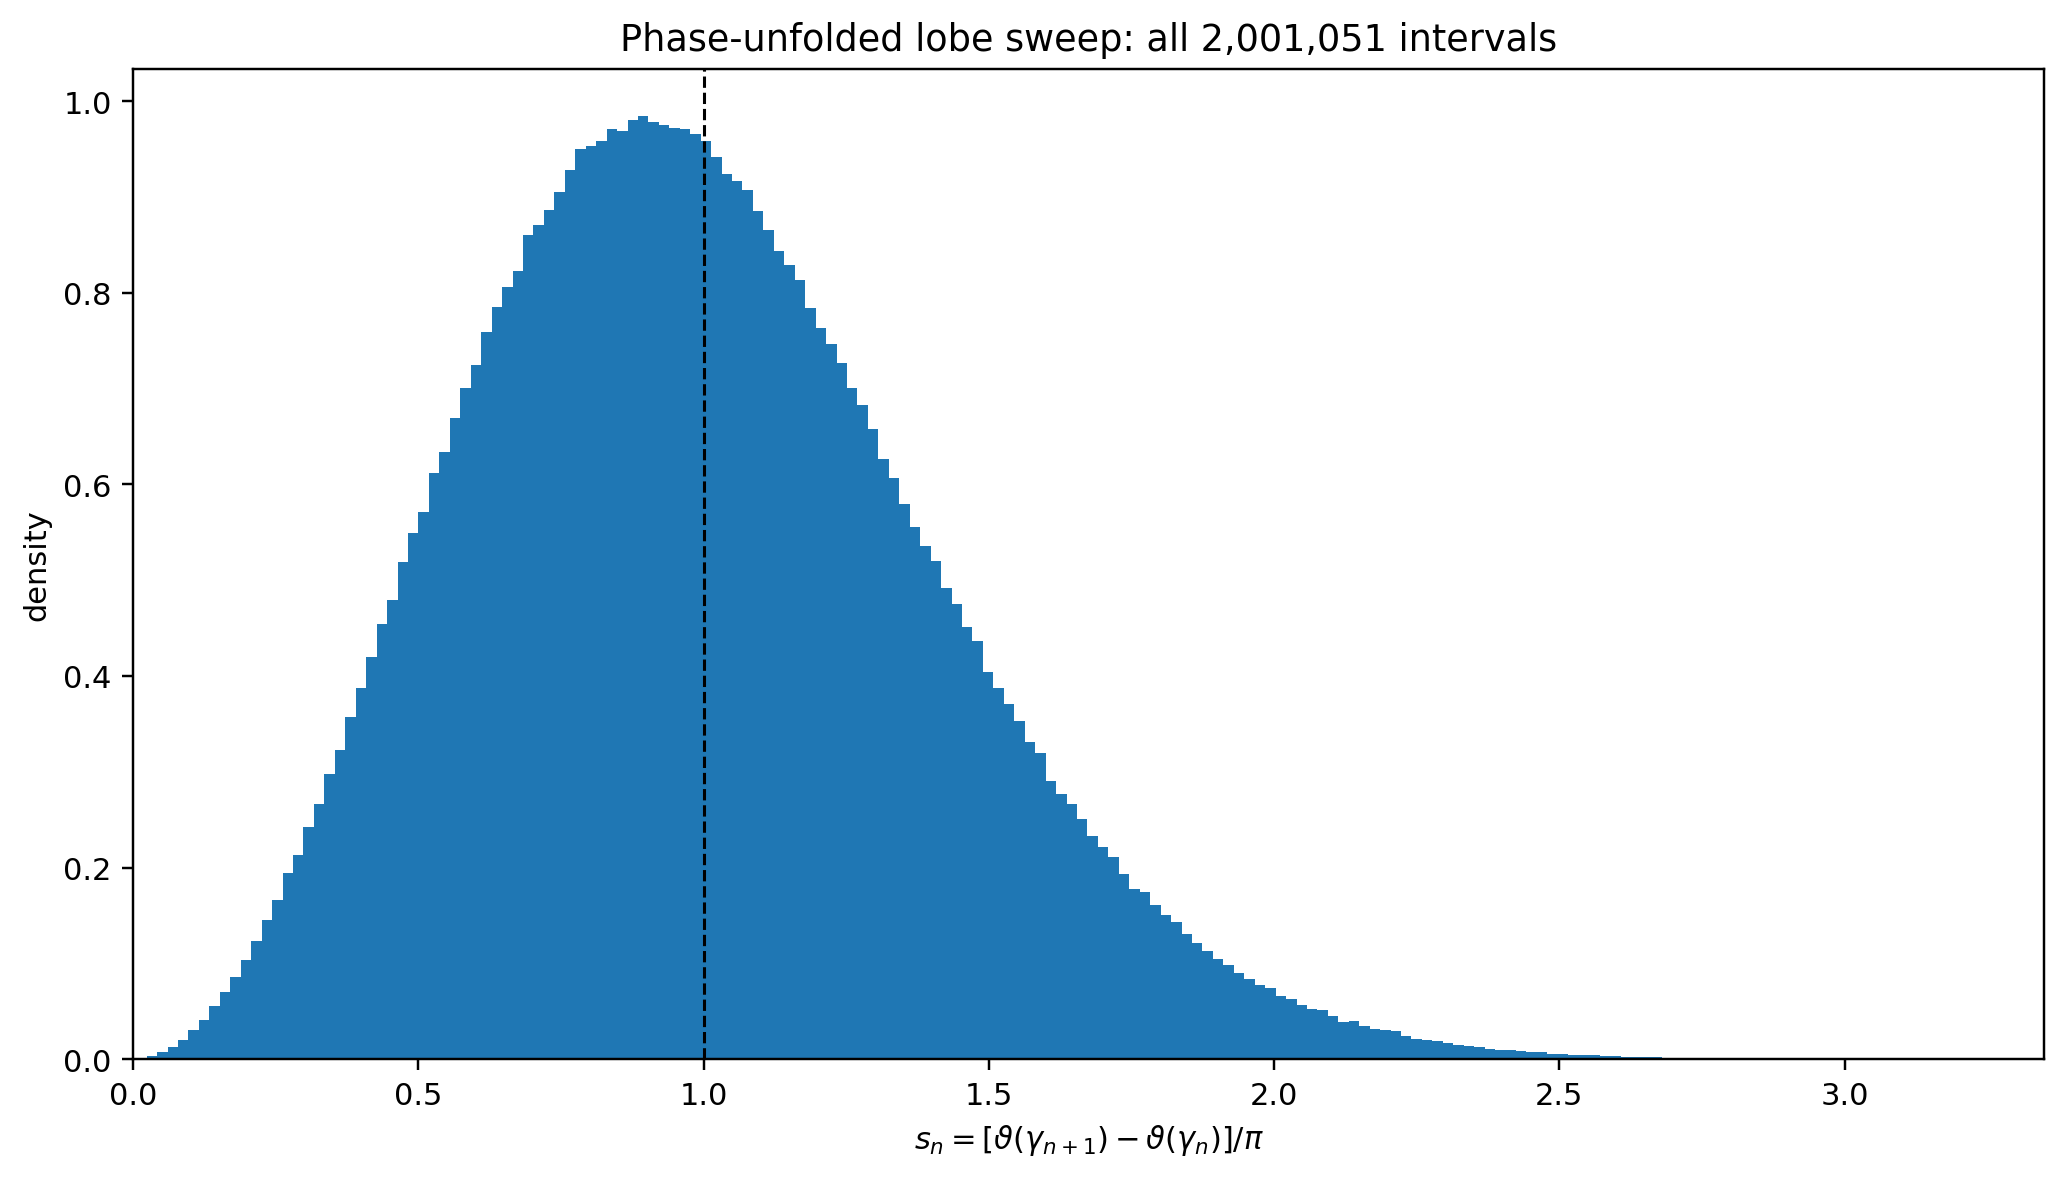
\includegraphics[width=\linewidth]{../figures/fig07_full_phase_spacing_histogram.png}
\caption{Phase-unfolded sweep distribution.}
\label{fig:full-phase-hist}
\end{subfigure}\hfill
\begin{subfigure}[t]{.47\textwidth}
\centering
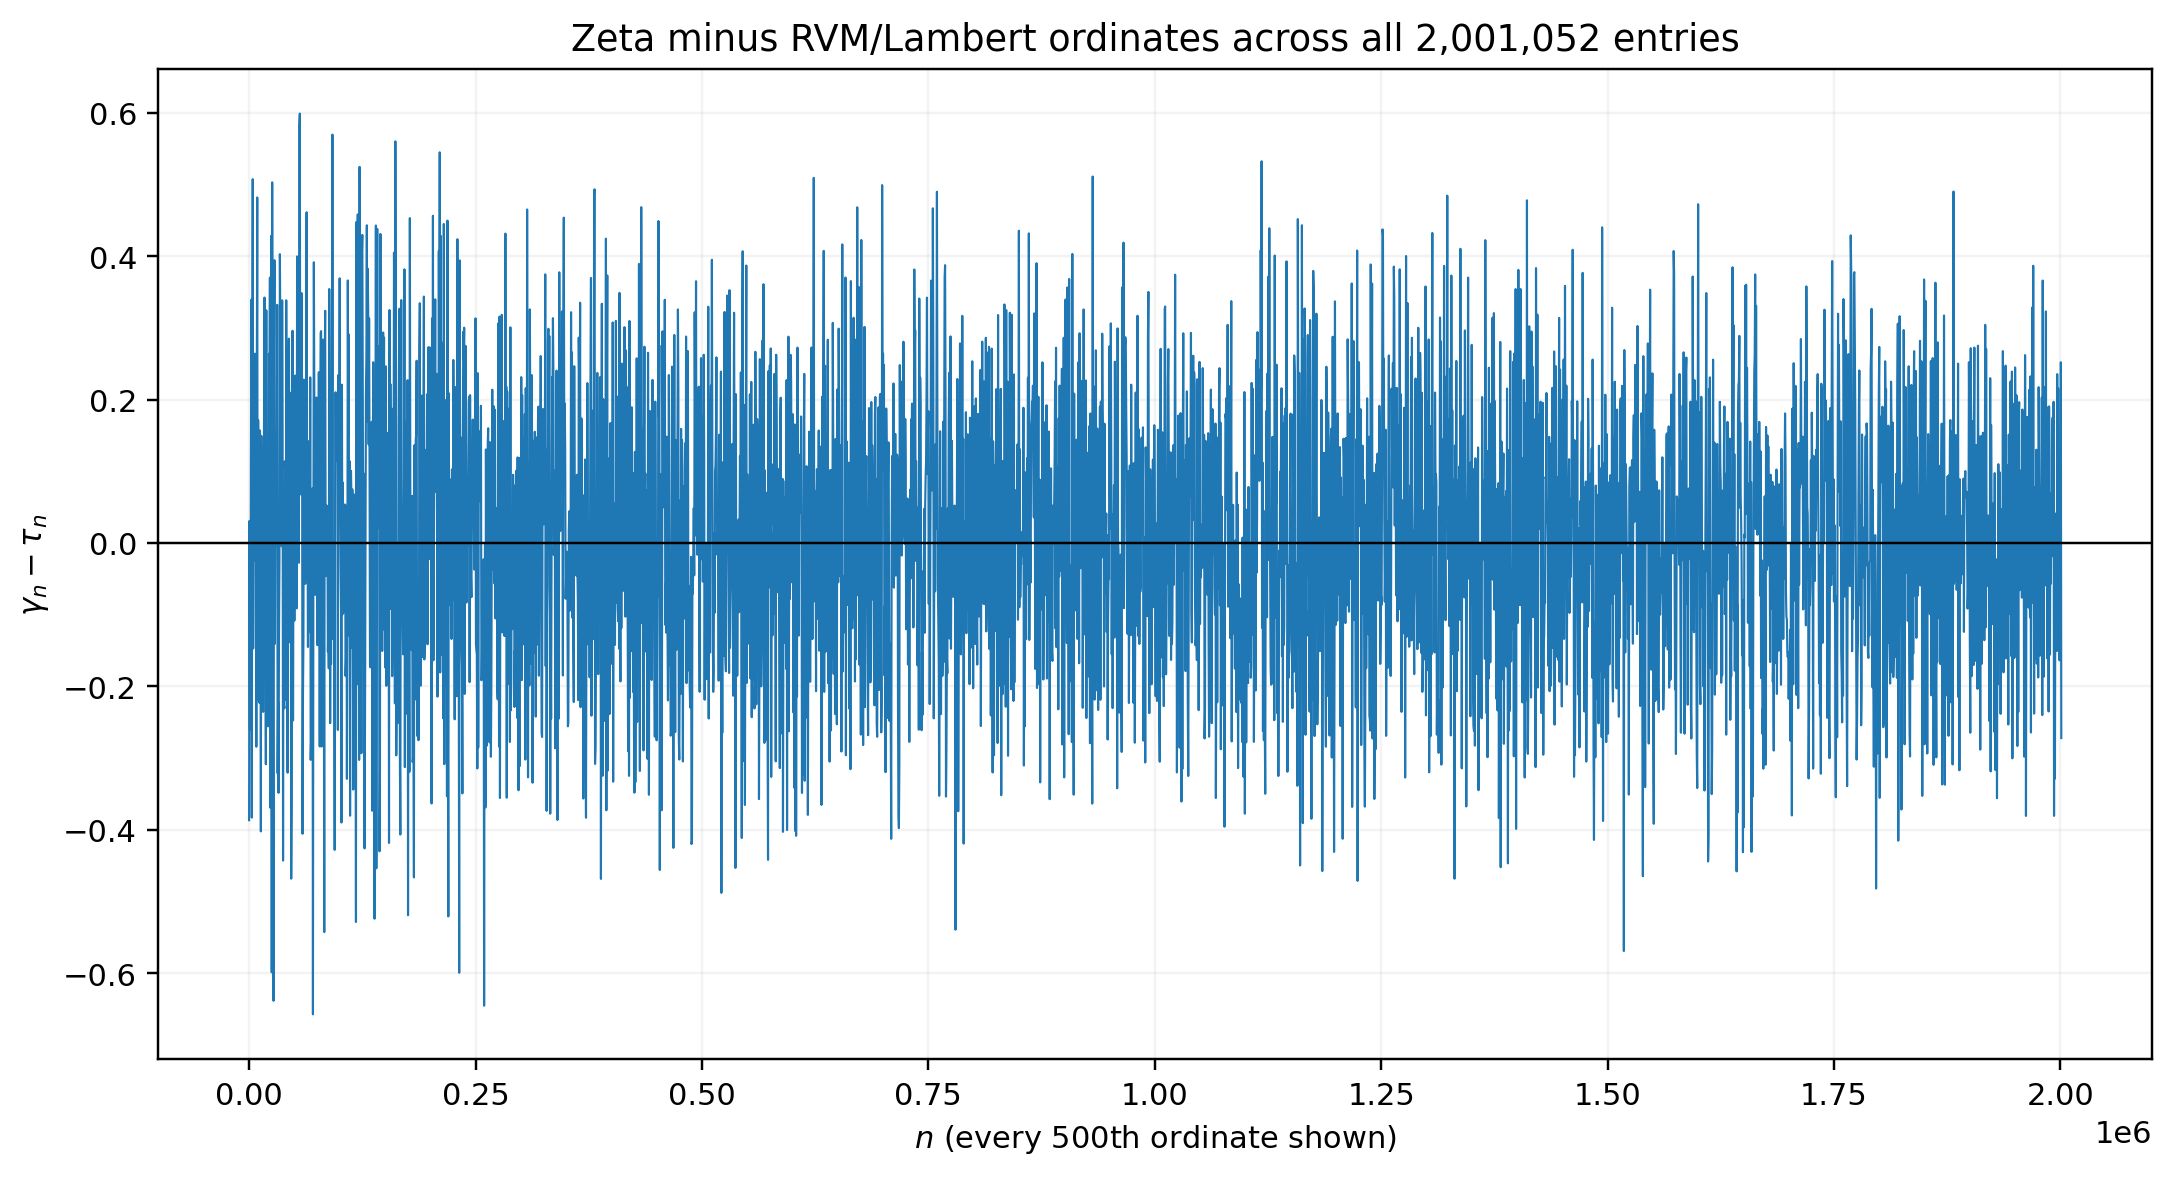
\includegraphics[width=\linewidth]{../figures/fig08_full_zeta_minus_rvm_lambert.png}
\caption{$\gamma_n-\tau_n$ over the complete carried corpus.}
\label{fig:full-rvm-diff}
\end{subfigure}
\caption{Global numerical diagnostics carried unchanged into Version 5.}
\label{fig:full-audit-pair}
\end{figure}

\section{What remains genuinely open in this construction}
\label{sec:open}

The exact RVM theorem, Theorem~\ref{thm:rvm-no-exit}, exhibits a complete no-exit mechanism for the tangent-circle skeleton.  The exact zeta lobes possess the same global quarter-turn equation \eqref{eq:quarter-turn}, but the deformation from the RVM skeleton is not currently controlled by an invariant strong enough to imply \eqref{eq:global-no-exit}.

The reciprocal chart does not alter the logical event by Proposition~\ref{prop:zero-pole-equivalence}.  The projective defect does not close the gap either: Remark~\ref{rem:Schwarzian-status} records that the Schwarzian moment identities recover endpoint holonomy but do not yet constrain it in a zero-excluding region.

Accordingly, the unresolved analytic target can be stated without introducing a new classical RH criterion:
\begin{multline}
\text{derive from the exact lobe geometry and }F_\delta=-iF_t\text{ a global invariant}\\
\text{that excludes }F=0\text{ for }\delta\neq0.
\label{eq:open-target}
\end{multline}
The target is first-order in the evolution variable; the missing ingredient is a global rigidity inequality or invariant of the specific zeta lobe family.

\section{Provenance of the construction}
\label{sec:provenance}

The zeta function, Hardy's $Z$-function, the Riemann--Siegel phase, the smooth Riemann--von Mangoldt phase, Lambert $W$, Cauchy--Riemann equations, Schwarzian derivatives, and variation of constants are classical ingredients.  Standard background on the zeta function is available in \cite{Titchmarsh1986,Edwards2001}; the Lambert $W$ reference used for the smooth inverse-counting parametrization is \cite{CorlessEtAl1996}.

The construction developed here keeps the three-dimensional trace \eqref{eq:Gamma-definition} as the primary object and organizes it into zero-to-zero lobes carrying Euclidean length, phase sweep, eccentricity, reciprocal scattering, and transverse quarter-turn dynamics.  The specific combination of the tangent-circle RVM skeleton, reciprocal straightening, endpoint-normalized lobe factorization, corrected scattering cocycle, and Schwarzian projective defect belongs to this program.

The two corrections incorporated in Version 5 are essential: the endpoint derivative identity is
\begin{equation}
\bigl(Y_n'(1)\bigr)^2=\frac{w_n'(1)}{w_n'(0)},
\label{eq:provenance-endpoint-correction}
\end{equation}
not its reciprocal, and the scattering potential is
\begin{equation}
Q_n=-\log a_n-i\psi_n,
\label{eq:provenance-Q-correction}
\end{equation}
which gives the modulus $a_{n+1}/a_n$ in the correct direction.

\section{Conclusion}
\label{sec:conclusion}

The Violet Thread is naturally described as a chain of eccentric zero-to-zero lobes rather than a helix centered on the zero axis.  A unit phase sweep combined with a one-arch radial profile gives an exact tangent circle.  The smooth RVM/Lambert construction realizes that geometry exactly and, after transverse continuation, has the explicit no-exit barrier \eqref{eq:M-barrier}.

In reciprocal coordinates the same model becomes a straight scattering branch.  This change of chart does not create a distinct zero problem: Proposition~\ref{prop:zero-pole-equivalence} identifies the reciprocal pole and the direct zero as the same event.  Its genuine role is to simplify the model geometry and to expose endpoint scattering quantities.

For exact zeta lobes, the corrected holonomy
\begin{equation}
\Hcal_n=\frac{a_{n+1}}{a_n}e^{-i(\Omega_n-\pi)}
\label{eq:conclusion-holonomy}
\end{equation}
and projective defect $\Pcal_n$ produce the exact chain
\begin{equation}
\Pcal_n
\longrightarrow
Y_n
\longrightarrow
\Ical_n
\longrightarrow
\lambda_n
\longrightarrow
\Hcal_n
\longrightarrow
\overline Q_n-\overline Q_{n+1}.
\label{eq:conclusion-chain}
\end{equation}
The chain is mathematically consistent after the reciprocal/sign corrections, but it is descriptive until an additional rigidity inequality is proved.  The analytic target therefore remains sharply defined inside the same construction: transfer the RVM no-exit mechanism to the exact lobe family using an invariant of the global first-order transverse flow.

\appendix

\section{Carried first-49 Euclidean arc table}
\label{sec:appendix-arc-table}

\small
\begin{longtable}{rrrrrrr}
\toprule
$n$ & $\gamma_n$ & $\gamma_{n+1}$ & $g_n$ & $L_n$ & $R_n$ & $s_n$\\
\midrule
\endfirsthead
\toprule
$n$ & $\gamma_n$ & $\gamma_{n+1}$ & $g_n$ & $L_n$ & $R_n$ & $s_n$\\
\midrule
\endhead
1 & 14.134725142 & 21.022039639 & 6.887314 & 10.366625 & 1.505177 & 1.120464 \\
2 & 21.022039639 & 25.010857580 & 3.988818 & 5.821954 & 1.459569 & 0.823387 \\
3 & 25.010857580 & 30.424876126 & 5.414019 & 11.347658 & 2.095977 & 1.277467 \\
4 & 30.424876126 & 32.935061588 & 2.510185 & 3.527308 & 1.405198 & 0.646207 \\
5 & 32.935061588 & 37.586178159 & 4.651117 & 11.313733 & 2.432477 & 1.276284 \\
6 & 37.586178159 & 40.918719012 & 3.332541 & 6.525882 & 1.958230 & 0.971574 \\
7 & 40.918719012 & 43.327073281 & 2.408354 & 3.954497 & 1.641991 & 0.729252 \\
8 & 43.327073281 & 48.005150881 & 4.678078 & 14.508230 & 3.101323 & 1.476437 \\
9 & 48.005150881 & 49.773832478 & 1.768682 & 2.558463 & 1.446537 & 0.577518 \\
10 & 49.773832478 & 52.970321478 & 3.196489 & 7.361974 & 2.303144 & 1.068877 \\
11 & 52.970321478 & 56.446247697 & 3.475926 & 10.542035 & 3.032871 & 1.197124 \\
12 & 56.446247697 & 59.347044003 & 2.900796 & 6.417297 & 2.212254 & 1.025228 \\
13 & 59.347044003 & 60.831778525 & 1.484735 & 2.134053 & 1.437330 & 0.533553 \\
14 & 60.831778525 & 65.112544048 & 4.280766 & 16.638613 & 3.886831 & 1.570144 \\
15 & 65.112544048 & 67.079810529 & 1.967266 & 3.718671 & 1.890273 & 0.736783 \\
16 & 67.079810529 & 69.546401711 & 2.466591 & 5.326509 & 2.159462 & 0.936736 \\
17 & 69.546401711 & 72.067157674 & 2.520756 & 6.712577 & 2.662922 & 0.971691 \\
18 & 72.067157674 & 75.704690699 & 3.637533 & 13.914973 & 3.825387 & 1.426798 \\
19 & 75.704690699 & 77.144840069 & 1.440149 & 2.176283 & 1.511151 & 0.572652 \\
20 & 77.144840069 & 79.337375020 & 2.192535 & 4.602265 & 2.099061 & 0.880017 \\
21 & 79.337375020 & 82.910380854 & 3.573006 & 15.382321 & 4.305148 & 1.454644 \\
22 & 82.910380854 & 84.735492981 & 1.825112 & 3.922717 & 2.149302 & 0.752565 \\
23 & 84.735492981 & 87.425274613 & 2.689782 & 6.941343 & 2.580634 & 1.120470 \\
24 & 87.425274613 & 88.809111208 & 1.383837 & 2.364722 & 1.708816 & 0.581616 \\
25 & 88.809111208 & 92.491899271 & 3.682788 & 17.699808 & 4.806089 & 1.564427 \\
26 & 92.491899271 & 94.651344041 & 2.159445 & 5.028165 & 2.328453 & 0.928236 \\
27 & 94.651344041 & 95.870634228 & 1.219290 & 1.792394 & 1.470031 & 0.527586 \\
28 & 95.870634228 & 98.831194218 & 2.960560 & 10.692946 & 3.611799 & 1.291244 \\
29 & 98.831194218 & 101.317851006 & 2.486657 & 9.200234 & 3.699841 & 1.095477 \\
30 & 101.317851006 & 103.725538040 & 2.407687 & 7.271512 & 3.020123 & 1.069947 \\
31 & 103.725538040 & 105.446623052 & 1.721085 & 3.359732 & 1.952101 & 0.770293 \\
32 & 105.446623052 & 107.168611184 & 1.721988 & 3.798904 & 2.206115 & 0.775172 \\
33 & 107.168611184 & 111.029535543 & 3.860924 & 21.415034 & 5.546608 & 1.753940 \\
34 & 111.029535543 & 111.874659177 & 0.845124 & 1.144932 & 1.354751 & 0.386799 \\
35 & 111.874659177 & 114.320220915 & 2.445562 & 6.361304 & 2.601163 & 1.124991 \\
36 & 114.320220915 & 116.226680321 & 1.906459 & 5.173808 & 2.713831 & 0.882782 \\
37 & 116.226680321 & 118.790782866 & 2.564103 & 10.900164 & 4.251064 & 1.195136 \\
38 & 118.790782866 & 121.370125002 & 2.579342 & 9.953938 & 3.859099 & 1.211127 \\
39 & 121.370125002 & 122.946829294 & 1.576704 & 2.933196 & 1.860334 & 0.744648 \\
40 & 122.946829294 & 124.256818554 & 1.309989 & 2.254766 & 1.721209 & 0.621133 \\
41 & 124.256818554 & 127.516683880 & 3.259865 & 18.008263 & 5.524235 & 1.555161 \\
42 & 127.516683880 & 129.578704200 & 2.062020 & 6.634166 & 3.217314 & 0.990584 \\
43 & 129.578704200 & 131.087688531 & 1.508984 & 3.163710 & 2.096582 & 0.728222 \\
44 & 131.087688531 & 133.497737203 & 2.410049 & 7.413230 & 3.075967 & 1.168789 \\
45 & 133.497737203 & 134.756509753 & 1.258773 & 2.604796 & 2.069315 & 0.613221 \\
46 & 134.756509753 & 138.116042055 & 3.359532 & 20.311522 & 6.045937 & 1.645739 \\
47 & 138.116042055 & 139.736208952 & 1.620167 & 3.702662 & 2.285358 & 0.798342 \\
48 & 139.736208952 & 141.123707404 & 1.387498 & 2.480013 & 1.787399 & 0.686072 \\
49 & 141.123707404 & 143.111845808 & 1.988138 & 5.929834 & 2.982606 & 0.986847 \\

\end{longtable}
\normalsize

\section{Carried first-49 eccentric-lobe table}
\label{sec:appendix-eccentric-table}

\scriptsize
\begin{longtable}{rrrrrrrr}
\toprule
$n$ & $s_n$ & $A_n$ & $\Ree\Ccal_n$ & $\Imm\Ccal_n$ & $E_n$ & $D_n$ & $E_n^{\mathrm{arch}}$\\
\midrule
\endfirsthead
\toprule
$n$ & $s_n$ & $A_n$ & $\Ree\Ccal_n$ & $\Imm\Ccal_n$ & $E_n$ & $D_n$ & $E_n^{\mathrm{arch}}$\\
\midrule
\endhead
1 & 1.120464 & 2.340551 & -0.197557 & -1.069503 & 0.929351 & 0.061686 & 0.937571 \\
2 & 0.823387 & 1.459266 & 0.213980 & -0.771070 & 1.096730 & 0.094567 & 1.082844 \\
3 & 1.277467 & 2.847473 & -0.467973 & -1.096033 & 0.837064 & 0.136510 & 0.850629 \\
4 & 0.646207 & 0.925523 & 0.288074 & -0.464831 & 1.181729 & 0.189896 & 1.153336 \\
5 & 1.276284 & 2.942394 & -0.569632 & -1.094018 & 0.838387 & 0.136454 & 0.851303 \\
6 & 0.971574 & 1.812834 & 0.081551 & -0.914154 & 1.012541 & 0.017313 & 1.014081 \\
7 & 0.729252 & 1.129621 & 0.254384 & -0.592648 & 1.141863 & 0.145029 & 1.122018 \\
8 & 1.476437 & 3.664837 & -0.863191 & -1.008247 & 0.724330 & 0.221013 & 0.734307 \\
9 & 0.577518 & 0.713345 & 0.269293 & -0.337016 & 1.209490 & 0.225516 & 1.176783 \\
10 & 1.068877 & 2.061177 & -0.181974 & -0.965993 & 0.953808 & 0.038440 & 0.964823 \\
11 & 1.197124 & 2.913512 & -0.382057 & -1.235552 & 0.887776 & 0.100247 & 0.895805 \\
12 & 1.025228 & 1.816095 & 0.036943 & -0.885544 & 0.976066 & 0.020841 & 0.987285 \\
13 & 0.533553 & 0.603289 & 0.243649 & -0.278203 & 1.225990 & 0.247800 & 1.190566 \\
14 & 1.570144 & 4.166936 & -1.145451 & -0.811102 & 0.673659 & 0.256740 & 0.678236 \\
15 & 0.736783 & 1.134191 & 0.276452 & -0.582461 & 1.136911 & 0.140711 & 1.119024 \\
16 & 0.936736 & 1.551068 & 0.058545 & -0.797230 & 1.030743 & 0.033477 & 1.030967 \\
17 & 0.971691 & 2.004530 & 0.001540 & -1.017693 & 1.015394 & 0.017383 & 1.014024 \\
18 & 1.426798 & 3.641859 & -0.733955 & -1.155689 & 0.751843 & 0.201781 & 0.763769 \\
19 & 0.572652 & 0.632316 & 0.243141 & -0.294845 & 1.208782 & 0.227034 & 1.178356 \\
20 & 0.880017 & 1.368228 & 0.081166 & -0.716356 & 1.053829 & 0.063916 & 1.057534 \\
21 & 1.454644 & 3.998567 & -0.963358 & -1.117642 & 0.738028 & 0.215416 & 0.747269 \\
22 & 0.752565 & 1.238064 & 0.280679 & -0.641532 & 1.131195 & 0.132691 & 1.112669 \\
23 & 1.120470 & 1.952783 & -0.142953 & -0.890642 & 0.923852 & 0.061227 & 0.937568 \\
24 & 0.581616 & 0.740985 & 0.267355 & -0.358679 & 1.207469 & 0.223290 & 1.175449 \\
25 & 1.564427 & 4.477141 & -1.231837 & -0.883265 & 0.677118 & 0.257169 & 0.681668 \\
26 & 0.928236 & 1.505698 & 0.160950 & -0.754544 & 1.024799 & 0.041524 & 1.035022 \\
27 & 0.527586 & 0.519217 & 0.212790 & -0.237095 & 1.227156 & 0.250352 & 1.192361 \\
28 & 1.291244 & 2.933506 & -0.671815 & -1.008007 & 0.825884 & 0.142695 & 0.842757 \\
29 & 1.095477 & 2.698327 & -0.166322 & -1.268317 & 0.948125 & 0.049823 & 0.950863 \\
30 & 1.069947 & 2.126243 & -0.049191 & -1.015659 & 0.956475 & 0.038085 & 0.964266 \\
31 & 0.770293 & 1.023117 & 0.211215 & -0.531506 & 1.118027 & 0.121926 & 1.105401 \\
32 & 0.775172 & 1.198408 & 0.196300 & -0.637329 & 1.112934 & 0.119259 & 1.103377 \\
33 & 1.753940 & 5.193290 & -1.310908 & -0.745479 & 0.580769 & 0.316608 & 0.567986 \\
34 & 0.386799 & 0.322351 & 0.169868 & -0.115712 & 1.275223 & 0.318951 & 1.229286 \\
35 & 1.124991 & 1.800191 & -0.233571 & -0.789519 & 0.914730 & 0.064462 & 0.935145 \\
36 & 0.882782 & 1.613611 & 0.134317 & -0.848048 & 1.064221 & 0.062578 & 1.056266 \\
37 & 1.195136 & 3.102800 & -0.465731 & -1.298326 & 0.889088 & 0.099593 & 0.896905 \\
38 & 1.211127 & 2.814119 & -0.287478 & -1.197322 & 0.875123 & 0.107082 & 0.888027 \\
39 & 0.744648 & 0.889614 & 0.215212 & -0.451735 & 1.124938 & 0.134423 & 1.115870 \\
40 & 0.621133 & 0.697945 & 0.218616 & -0.350456 & 1.183625 & 0.200187 & 1.162160 \\
41 & 1.555161 & 4.592177 & -1.304854 & -0.865631 & 0.681975 & 0.254118 & 0.687228 \\
42 & 0.990584 & 2.022093 & 0.093840 & -1.006610 & 0.999929 & 0.016746 & 1.004694 \\
43 & 0.728222 & 1.004221 & 0.238322 & -0.521409 & 1.141767 & 0.145333 & 1.122426 \\
44 & 1.168789 & 2.097730 & -0.245463 & -0.908151 & 0.896912 & 0.084512 & 0.911408 \\
45 & 0.613221 & 0.869925 & 0.288251 & -0.432411 & 1.194770 & 0.206969 & 1.164882 \\
46 & 1.645739 & 5.050324 & -1.375512 & -0.819209 & 0.634011 & 0.287141 & 0.632816 \\
47 & 0.798342 & 1.168116 & 0.240775 & -0.593840 & 1.097143 & 0.106380 & 1.093630 \\
48 & 0.686072 & 0.758449 & 0.203407 & -0.389108 & 1.157800 & 0.166754 & 1.138697 \\
49 & 0.986847 & 1.799303 & -0.062979 & -0.895959 & 0.998353 & 0.019753 & 1.006548 \\

\end{longtable}
\normalsize

\section{Reproducibility package}
\label{sec:appendix-reproducibility}

The archive contains one principal TeX source, its compiled PDF, the fifteen PNG files actually used by the manuscript, the consolidated Python analysis script from the preceding verified computation, the carried CSV/TeX outputs, and the two binary ordinate files.  The binary files are copied unchanged into Version 5 and are not read by the Version 5 revision process.

\begin{thebibliography}{9}

\bibitem{Titchmarsh1986}
E. C. Titchmarsh, revised by D. R. Heath-Brown,
\emph{The Theory of the Riemann Zeta-Function}, 2nd ed.,
Oxford University Press, Oxford, 1986.

\bibitem{Edwards2001}
H. M. Edwards,
\emph{Riemann's Zeta Function},
Dover Publications, Mineola, NY, 2001.

\bibitem{Montgomery1973}
H. L. Montgomery,
\emph{The pair correlation of zeros of the zeta function},
in \emph{Analytic Number Theory}, Proc. Sympos. Pure Math. \textbf{24},
American Mathematical Society, Providence, RI, 1973, pp. 181--193,
doi:10.1090/pspum/024/9944.

\bibitem{CorlessEtAl1996}
R. M. Corless, G. H. Gonnet, D. E. G. Hare, D. J. Jeffrey, and D. E. Knuth,
\emph{On the Lambert W function},
Adv. Comput. Math. \textbf{5} (1996), 329--359,
doi:10.1007/BF02124750.

\end{thebibliography}

\end{document}
